%%%%%%%%Bilecik �eyh Edebali �niversitesi M�hendsilik Fak�ltesi%%%%
%%%%%%%%%%%Bilgisayar M�hendisli�i Proje I-II �al��mas�%%%%%%%%%%%%
%%%%%%%%%%%%%%%%%%%%%%LaTeX Class%%%%%%%%%%%%%%%%%%%%%%%%%%%%%%%%%%
\documentclass{BUP}
%%%%%%%%%%%%%%%%%%%%%%%%%%%%%%%%%%%%%%%%%%%%%%%%%%%%%%%%%%%%%%%%%%%%%%%%%%%
\begin{document}
\shorthandoff{=}%grafik komutlar�nda babelden kaynaklanan hatay� engeller.
%%%%%%%%%%%%%Proje I-II �al��malar�n�n B�l�mleri%%%%%%%%%%%%%%%%%%%%%%%%%%%
\thispagestyle{empty} %Bu sayfaya sayfa numaralar� yaz�lmaz
\begin{figure}[H]
\centering

\includegraphics[scale=0.2]{logomuz}
%Bu komutla resim dosyam�z� y�kl�yoruz.
\end{figure}
%sa�a 4 sol 2 a�a�� yukar� 3%
\begin{center}
\textbf{T.C.}\\
\textbf{B�LEC�K �EYH EDEBAL� �N�VERS�TES�}\\
\textbf{M�HEND�SL�K FAK�LTES�}

\textbf{B�LG�SAYAR M�HEND�SL��� B�L�M�}
\end{center}

\vspace*{4cm}%bir miktar bo�luk b�rakmak i�in
\begin{center}
\textbf{BULUT TABANLI G�R�NT� ��LEME}

\textbf{ZEYNEP KOTAN}

\textbf{PROJE II �ALI�MASI}
\end{center}

\vspace*{\fill}
\begin{center}
\textbf{PROJE II DANI�MANI : ��r. G�r. YUSUF MU�TU}

\textbf{B�LEC�K}\\ 
\textbf{\today}
\end{center}

\thispagestyle{empty} %Bu sayfaya sayfa numaralar� yaz�lmaz

\begin{figure}[H]
\centering

\includegraphics[scale=0.2]{logomuz}
%Bu komutla resim dosyam�z� y�kl�yoruz.
\end{figure}
%sa� 4 sol 2 a�a�� yukar� 3%
\begin{center}
\textbf{T.C.}\\
\textbf{B�LEC�K �EYH EDEBAL� �N�VERS�TES�}\\
\textbf{M�HEND�SL�K FAK�LTES�}

\textbf{B�LG�SAYAR M�HEND�SL��� B�L�M�}
\end{center}

\vspace*{4cm}%bir miktar bo�luk b�rakmak i�in
\begin{center}
\textbf{BULUT TABANLI G�R�NT� ��LEME}

\textbf{ZEYNEP KOTAN}

\textbf{PROJE II �ALI�MASI}
\end{center}

\vspace*{\fill}
\begin{center}
\textbf{PROJE I DANI�MANI : ��r. G�r. YUSUF MU�TU}

\textbf{B�LEC�K}\\ 
\textbf{\today}
\end{center}

\pagenumbering{roman}%romen rakamlar� kullan�lmaya ba�lan�yor.
\setcounter{page}{2}% sayfa numaras�n� ii'den ba�lat�l�yor.
\centerline{\bf �ZET}
\addcontentsline{toc}{section}{�ZET}
\begin{center}
\textbf{Projenin Amac�}
\end{center} 

\qquad Restaurant mobil uygulas�, restaurantta ki i�leri geli�tirmek ve hizmetleri m��teriye ula�t�rmak i�in en etkili ve en yeni yollardan biridir. Mobil uygulamaya sahip olman�n restaurant i�in y�zlerce faydas�ndan bahsedilebilir. Daha fazla m��teri kazanmak, mevcut m��terileri korumak, �r�nleri daha iyi anlat�p, g�sterebilmek i�in ki�iselle�tirilmi� bir alana sahip olmak, restaurant�n de�erini art�rmak, en son indirimlerden m��terileri haberdar etmek, m��teri sadakati sa�lamak, verimlili�i art�rmak, i�letme i�in direk pazarlama kanal� olu�turmak, rakiplerinden ayr��mak, marka olmak gibi y�zlerce neden s�ralanabilir.

\qquad Ya�am alanlar�m�zda art�k her �ey teknolojik oldu�undan bu uygulama bir nevi �a�a ayak uydurmaya olanak sa�layacak.


\begin{center}
\textbf{Projenin Kapsam�}
\end{center}
 \qquad Android studio kullan�larak geli�tirilen bu uygulama �imdilik sadece Android ��letim Sistemi olan cihazlarda �al���r. Restorant i�erisinde, m��terilerin sipari�ini verme ve sipari�ine
ula�ma s�recini otomatize ederek, ilgili s�reci m�mk�n mertebe optimize eden, h�zland�ran ve maliyet d���ren ��z�mler �retmektir.

\qquad G�rsel ve teknik yap�s�yla m��terilerinin karar verebilmesini kolayla�t�r�p ve restaurant�n hizmetlerini en iyi �ekilde m��terisine ula�t�rmas�n� sa�lar.


%%%%%%%%%%%%%%%%%%%%%%%%%%%%%%%%%%%%%%%ABSTRACT%%%%%%%%%%%%%%%%%%%%%%%%%%%%%%%%%%%%%%%%%%
\newpage
\centerline{\bf ABSTRACT}
\addcontentsline{toc}{section}{ABSTRACT}
\begin{center}
\textbf{Project Objective}
\end{center}

\qquad Restaurant mobile application is one of the most effective and newest ways to develop business in restaurant and deliver services to customers. Having a mobile application can be mentioned with hundreds of benefits for the restaurant. To gain more customers, to protect existing customers, to have a personalized space to better explain and display the products, to increase the value of the restaurant, to inform customers about the latest discounts, to provide customer loyalty, creating a direct marketing channel for the business, separating from its competitors, being a brand, etc.

\qquad Since everything in our living spaces is technological now, this practice will allow us to adapt to a kind of era.


\begin{center}
\textbf{Scope of Project}
\end{center}
 \qquad Developed using Android studio, this app currently only works on devices with the Android OS. Within the restaurant, customers can order and place orders
automating the process of reaching, optimizing the process to the extent possible, accelerating and cost-reducing solutions to produce.

\qquad Its visual and technical structure makes it easy for customers to make decisions and enables the restaurant to reach its customers in the best way possible.



\section*{TE�EKK�R}
Bu projenin ba��ndan sonuna kadar haz�rlanmas�nda  eme�i bulunan ve 
beni bu konuya y�nlendiren sayg�de�er hocam ve dan��man�m Say�n ��r. G�r. S�leyman UZUN'a t�m katk�lar�ndan ve hi� eksiltmedi�i deste�inden dolay� te�ekk�r ederim.
\vspace{2cm}

\begin{flushright}
\textbf{Zeynep KOTAN}

\today
\end{flushright}
\tableofcontents%bu komutun oldu�u yerde i�indekiler olu�turulur.



\pagenumbering{arabic}%Sayfa numaralamas�n� arap rakamlar�yla yapar.
\setcounter{page}{1}%sayfa numaras�n� 1'den ba�lat�r.
\section{G�R��}

Bu uygulama ile restaurant alan�nda yeni bir �a� ba�lat�lm�� oluyor. Restaurant mobil uygulamas� ile kaliteyi artt�rarak, m��terilere daha y�ksek standartlarda hizmet sunabilir, restaurant�n tan�t�m�n� daha etkili y�ntemle yapma olana��na sahip olunur. Ayr�yeten b�yle teknolojik uygulamalar g�n�m�zde daha ilgi �ekti�inden daha �ok insana hitap eden bir uygulamad�r.

M��teri restauranta geldi�inde her masaya �zel olarak konulan tabletlerden garsonun gelip sipari� almas�na gerek duymadan istedikleri sipari�i verebilir, sipari�inin ne kadar tuttu�unu  kasaya gitmeden �nce bilip ona g�re kendini haz�rlar.

��letmeci a��s�ndan bakacak olursak daha az garson ile daha az masraf olaca��ndan daha fazla kar etme olana��na sahiptir.


�al��anlar a��s�ndan ise daha az i� y�k� olaca��ndan bu uygulama �al��ma hayat�n� her a��dan kolayla�t�r�r.

Android Studio, Intelij IDEA'ya dayal� olup Android geli�tirme i�in �zel olarak tasarlanm�� android i�in resmi t�mle�ik geli�tirme ortam�d�r. Android uygulamalar�n�n geli�tirildi�i, �st seviye �zelliklere sahip ve Google taraf�ndan da �nerilen resmi programlama arac�d�r.

PhpMyAdmin, PHP ile yaz�lm��  a��k kaynak kodlu bir ara�t�r. Ba�l�ca kullan�m amac� internet �zerinden MySQL veritaban� y�netimidir. PhpMyAdmin'de olu�turdu�umuz veritaban�nda kay�tl� personel bilgisi, �r�nler, sipari�ler ve masalar  yer almaktad�r.


Veritaban� ve uygulama aras�ndaki ba�lant�y� da Sublime Text yard�m�yla olu�turdu�umuz PHP kodlar�yla web service yaz�ld�. Bu uygulama ile restaurant alan�nda yeni bir �a� ba�lat�lm�� oldu. Restaurant mobil uygulamas� ile kaliteyi artt�rarak, m��terilere daha y�ksek standartlarda hizmet sunabilir,restaurant�n tan�t�m�n� daha etkili y�ntemle yapma olana��na sahip olundu.




\section{BULUT TEKNOLOJ�S� NED�R?}\label{S:2}
Bu b�l�mde kullan�lan materyal ve metodlardan bahsedilecektir. Projede kullan�lan materyaller:
\begin{itemize}
\item Android Studio
\item PhpMyAdmin
\item Sublime Text
\item XAMPP
\end{itemize}
Se�ilen materyallerin neden se�ildi�i hakk�nda k�saca bilgilendireyim. Android Studio Android platformlarda uygulama geli�tirmek i�in gereklidir. Ba�ka bir IDE olup olmad���yla ilgili bilgi yoktur. Veritaban� i�in her platformdan eri�im sa�lanabilecek olmas� gerekti�i i�in PhpMyAdmin kullan�ld�. Php kodlar�n� derlemek i�in ise Sublime Text edit�r� kullan�ld�. Bunun yan�s�ra localhost(yerel sunucu) �zerinde php �al��t�rmak i�in Xapp program� kullan�ld�.
\subsection{Android Studio}\label{ss:1}

\textbf{Android Studio}, Android uygulamalar�n�n geli�tirildi�i, �st seviye �zelliklere sahip ve Google taraf�ndan da �nerilen resmi programlama arac�d�r. 
Android Studio, Android uygulama geli�tiricileri i�in tasarlanan olduk�a geni� kapsaml� ve �cretsiz programd�r. Program beraberinde bir �ok Android geli�tirici arac�yla birlikte gelmektedir.

Kar���k problemleri kolayca ��zmeyi sa�layabilecek olan Android Studio ile sadece uygulama geli�tirme de�il ayn� zamanda varolan uygulamalardaki sorunlar� ��zme i�lemleride ger�ekle�tirilebiliyor.

B�y�k ve geni� kapsaml� bir program olan Android Studio, Android geli�tiricilerinin i�lemlerini kolayla�t�rmak ve onlara kar��la�t�klar� sorunlarda yard�m etmek amac�yla Google taraf�ndan haz�rlanan ba�ar�l� ve etkileyici bir programd�r. Android Studio'nun kod geli�tiricilere sundu�u temel �zellikler �unlard�r:
\begin{itemize}
\item Gradle tabanl�, esnek proje in�a sistemi,
\item Farkl� �zellik ve s�r�mlere g�re �oklu APK ��kt�s�,
\item Temel proje �ablonlar�yla h�zl� ve kolay proje �retimi.
\item Ekran tasar�mlar�n� kolayla�t�ran s�r�kle-b�rak �zellikli zengin edit�r,
\item Uygulaman�n performans�, kullan�labilirli�i, farkl� s�r�mlerde �al��abilirli�inin kontrol edebilece�i test ara�lar�,
\item Kolay ve g�venli APK imzalanmas�,
\item Ek u�ra�a gerek kalmadan Google hizmetlerini uygulamaya ekleyebilmedir[1].
\end{itemize}
Andoid Studio bu proje i�in ana temeldir. Burada uygulama tasar�mlar� ve uygulama da istenen  (veritaban�ndaki) bilgiler �ekilir ve hangi i�lem ger�ekle�ti�inde �ekilmesi gerekti�i yer al�r.
\subsection{Sublime Text}\label{ss:2}
Sublime text edit�r� multiplatform bir edit�rd�r. Os X, Windows ve Linux sistemlerinde 32 ile 64 bit olarak kullan�l�r.

Sublime Text edit�r�, ho� kullan�c� aray�z� ile bir edit�rden beklenilenden fazlas�n� vermektedir.

Performans� ve inan�lmaz �zellikleri ile kullananlar�n bir daha vazge�emeyece�i t�rden bir edit�rd�r.  Macro kaydetme, d�zenli ifadeler ile arama metodu, �oklu se�im fonksiyonu ile ayn� anda d�zenleme imkan� ve dahas�n� kulland�k�a ke�fedece�iniz �zelliklerin hepsi "Sublime" text edit�r�nde mevcuttur[2].

Sublime Text Androidde yaz�lan verilerin �ekilebilmesi/al�nabilmesi i�in bir ara�t�r. Asl�nda tam olarak hangi bilginin nas�l �ekilip veya al�nmas�na karar verilen k�s�md�r. Bu karar Php kodlar�yla yaz�ya d�k�l�r ve istenilen i�lem ger�ekle�tirilir.

\subsection{PhpMyAdmin}\label{ss:3}
PhpMyAdmin, PHP ile yaz�lm�� a��k kaynak kodlu bir ara�t�r. Ba�l�ca kullan�m amac� �nternet �zerinden MySQL veritaban� y�netimidir.  Veritaban� olu�turma ve silme, tablo ekleme/de�i�tirme/silme, alan ekleme/de�i�tirme/silme, SQL sorgular� �al��t�rma, kullan�c�lar�, yetkileri ve alan anahtarlar�n� y�netme gibi i�levleri yapabilen bedava yaz�l�md�r.

Ayr�ca phpMyAdmin, ilk s�r�m�nden k�sa bir s�re sonra b�y�k bir kullan�c� ve geli�tirici kitlesinin ilgisini kazanan phpMyAdmin, zaman�nda en pop�ler PHP uygulamalar�ndan biri haline gelmi�tir.

PhpMyAdmin, Android'de yaz�lan uygulaman�n istedi�i veriyi verir. Ama bu iki uygulama birbirinin dilinden anlamad��� i�in burada Sublime Text devreye girer ve birbirlerini anlamalar�n� sa�lar. Bu �ekilde de PhpMyAdminden bilgiler al�n�r.


\textbf{PhpMyAdmin Ne ��e Yarar?}
\begin{itemize}
\item Veritaban� a��l�r,
\item Kullan�c� tan�mlan�r,
\item Tablolar olu�turulur,
\item Tablolara veri ekleme, silme,  d�zenleme, optimize etme,
\item Veritabanlar�n�n yede�ini alma ve yede�ini a�abilme,
\item Txt dosyas�ndan SQL kodlar�n� okuyup �al��t�rma,
\item Tablolarda yeni alan a�ma ve istedi�in alan� silme,
\item Veritaban�n�n optimize edilmesi,
\item Veritaban�na SQL sorgular� g�nderme,
\item Veritaban�n� ba�ka bir isimle �o�altma

ve benzeri i�lemler yap�labilmektedir[3].
\end{itemize}

\subsubsection{PHP Nedir?}\label{ss:4}
PHP k�saca web tabanl� bir programlama dilidir. Eskiden a��l�m� "Personel Home Page" yani ki�isel anasayfa iken g�n�m�zde geli�mesi ve daha iyi anlam kazanmas� ile "PHP:Hypertext Preprocessor" yani �st�n Yaz� �nlemcisi olmu�tur.

Di�er web tabanl� dillere g�re onlarca avantaj� olan ve g�n�m�zde en popiler olan dillerden birisidir. �nternet �zerindeki dura�an sabit yaz�lara dinamiklik katmay� sa�layan bir web tabanl� dil olan PHP, en iyi performans� MYSQL veritaban� ve Linux i�letim sistemi ile g�sterir.

1995 y�l�nda Rasmus Lerdorf taraf�ndan olu�turulan PHP g�n�m�zde halen geli�tirilmesine devam edilmekte ve en son s�r�m� PHP5 olmas�yla beraber tamamen a��k kaynakl� ve �cretsizdir.

Neden PHP:
\begin{itemize}
\item A��k kaynakl� bir dil olmas� ve en �nemlisi �al��mas� i�in y�ksek donan�m ya da �cretli yaz�l�mlara ihtiya� duymamas� nedeniyle PHP yaz�l�mlar� olduk�a d���k �cretlerde bar�nd�r�labilir.
\item Bir �ok geli�mi� platformda sorunsuz olarak �al���rken ayn� zamanda  geli�mi� di�er teknolojilerle(�rne�in MYSQL) uyumlu olarak �al��abilir.
\item Dil yap�s�, kodlamas� ve kullan�m� di�er dillere nazaran olduk�a daha kolayd�r.
\item Son derece h�zl� bir dildir[4].
\end{itemize}

\subsection{XAMPP}\label{ss:3}
%Xampp program� localhost(yerel sunucu) �zerinde php �al��t�rmak i�in kullan�l�r. PHP yazmak i�in wamp server'a alternatif olarak g�sterilebilir. Xampp MySQL, Apache gibi servislere eklenti eklemeye,  rahatl�kla kontrol etmeye olanak sa�lar. Kullan�m� gayet basittir[8].
%
Geli�tiricilerin �zerinde �al��t�klar� projeleri i�in, kolay bir �ekilde yerel web sunucusu olu�turmalar�n� sa�layan, bir apache da��t�m�d�r. Xampp, kelimesinde her harfin bir anlam� vard�r. X:�apraz platform, A:apache, M:mysql, P:php ve son P harfi de perl anlam�na gelmektedir. Yukar�da web sunucusunu kolay bir �ekilde olu�turmam�z� sa�l�yor dememizde ki neden ise bir web sunucusu i�in gerekli olan b�t�n bile�enleri paket halinde bize sunmas�d�r. �apraz platform da nedir diye soran arkada�lar� da cevaps�z b�rakmayal�m. �apraz platform; windows, mac ve linux i�letim sistemlerinde neredeyse ayn� performans� sergileyerek �al��t��� anlam�na gelmektedir[5].
  




\section{PROJE'N�N TASARIM A�AMALARI}\label{S:3}
Bu b�l�mde yap�lan ilk olarak uygulaman�n veritaban� k�sm�ndan bilgiler verilecektir. �kinci olarak  uygulaman�n yaz�ld��� program ve veritab�n� biribirine ba�layan Php kodlar�ndan bahsedilecektir. ���nc� olarakta uygulamay� olu�tururken kar�� kar��ya kal�nan hatalardan bahsedilecektir. Ve son olarakta uygulaman�n ekran g�r�nt�s� konularak bu sayfalar�n ne ama�la yap�ld���na dair k�sa bilgilendirmeler yap�lacakt�r.
\subsection{Veritaban� }\label{ss:1}
\qquad Veritaban� olarak PhpMyAdmin kulaln�lmas�n�n sebebi internet �zerinden MYSQL veritaban� y�netimidir.

\qquad  Bu program arac�l��� ile veritaban�nda tablo olu�turup,  tablolar� silebilir, i�erisindeki verileri bo�altabilir veya ilgili tablo verisini g�ncelleyip,  d�zenlenebilir. Asl�nda bu c�mle o kadar �ok uzat�labilir ki. Veritaban� ile ilgili akla gelebilecek her t�rl� i�lemi phpmyadmin ad� verilen program sayesinde yap�labilir. Sadece veri giri� i�lemlerini ve baz� sorgulamalar� web sayfalar�ndaki aray�zler sayesinde ger�ekle�tirilir. Bunun haricinde arka planda har�l har�l �al��an bu muazzam yap�lara do�rudan ula�mak istenilirse phpmyadmin veya bu program muadilinde bir ba�ka veritaban� y�netim program�na ihtiya� olacakt�r.Bu projede XAMPP kullan�lmaktad�r. 
 
\qquad  Bu proje i�in PhpMyAdmin ve Android Studio birbirine ba�lanarak kullan�lacakt�r.
 
 \qquad Php kullan�lmas�ndaki sebep ise personel bilgilerinin yer almas� ve uygulaman�n g�venli�inin artt�r�lmak istenmesidir.Php kodlar�n�n yaz�lmas� i�in tercih edilen Sublime Text'dir.
 

 \subsubsection{Veritaban�na Giri�}
 Proje i�inde kullan�lacak olan veri taban�n� olu�turmak i�in PhpMyAdmin'e giri� yap�larak veritaban� olu�turulmu�tur. �ekil 4'te giri� sayfas� g�r�lmektedir.
 
 
 
\begin{figure}[H]
\centering
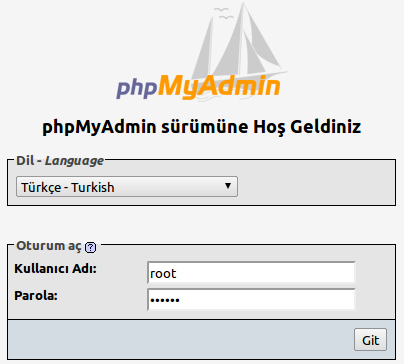
\includegraphics[scale=0.3]{php}
%Bu komutla resim dosyam�z� y�kl�yoruz.

\centering
�ekil 4:Veritaban�na Giri�
\end{figure}


Buradan giri� yap�larak yeni bir restaurant ad�nda veritaban� olu�turuldu. Olu�turulan veritaban�  d�rt tablodan olu�maktad�r. Bunlar; �r�nler, sipari�ler, personel ve masalar tablolar�d�r. �r�nler tablosunun i�erisinde men�de bulunan yemek isimleri, kategorileri ve fiyat bilgileri bulunmaktad�r. Personel tablosunda ise personel ad�, soyad� , telefonu, emaili ve sisteme giri� yapaca�� zaman gerekli olan �ifre bilgisi yer almaktad�r. Masalarda ise masano bilgisi tutulmaktad�r. Sipari� tablosundaysa masano, sipari� detay� ve toplam tutar yer almaktad�r.Veritaban� tablolar� �ekil 5'te g�r�lmektedir.

 
 \begin{figure}[H]
 
 
\centering
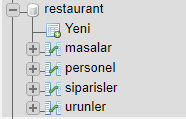
\includegraphics[scale=0.8]{restaurant}
%Bu komutla resim dosyam�z� y�kl�yoruz.

\centering
�ekil 5:Veritaban� Tablolar�
\end{figure}


 \subsubsection{Veritaban�na Tablo Ekleme}
 
 Olu�turulan veritaban�ndaki tablolara veri  ekleyerek uygulamada kullanaca��m�z alanlar olu�turuldu. �ekil 6'da olu�turulan �r�n tablosunun s�tunlar�  g�r�lmektedir.
 
\begin{figure}[H]
\centering
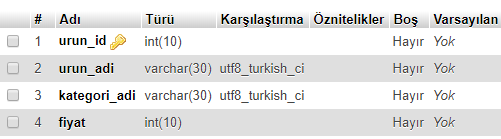
\includegraphics[scale=0.8]{sekil6}
%Bu komutla resim dosyam�z� y�kl�yoruz.

\centering
�ekil 6:�r�n Tablosu
\end{figure}
 
  
   \subsection{Php �le Ba�lant�}\label{ss:2}
Php kodlar� ile  veitaban�na ba�lanarak Android Studio'da istenen veriler �ekilir. Burada uygulama geli�tiricilerin bildi�i ama bu i�e yani ba�layan insanlar�n kar��t�rd��� bir durum vard�r. Php ile veritaban�ndan bilgiyi �ekip Android Studio'ya aktarabilece�imiz gibi   Android Studio'dan bilgi �ekip veritaban�na da aktarma yap�labilir.  
  \subsubsection{Men� Sayfas�} 
 Uygulama ile veritaban�na ba�lan�l�r.  Sonra m��teriler i�in men� k�sm� devreye girer ve se�ilen  kategoriye g�re veritaban�nda kay�tl� bilgi yoksa sistem hata mesaj� verir. Var ise sistem ba�lat�lm�� olur.Olu�turulan bu php dosyas�n� siteye y�kledikten sonra men� sayfas�n�n tasar�m�na ge�ilir.
   \begin{figure}[H]
\centering

\includegraphics[scale=0.7]{a}
%Bu komutla resim dosyam�z� y�kl�yoruz.

\centering

Bu �ekilde veritaban�na ba�lant�s� ger�ekle�tirilir.
\end{figure}

Ba�lant� ger�ekle�tikten sonra Android Studio'da se�ilen karatere g�re veritaban�ndaki �r�n �ekilir. 
     \begin{figure}[H]
\centering

\includegraphics[scale=0.7]{b}
%Bu komutla resim dosyam�z� y�kl�yoruz.

\centering
Se�ilen kategoriye g�re �r�n tablosundaki �r�n �ekilir.
\end{figure}

  
     \subsubsection{Mutfak Sipari� Sayfas�}\label{ss:6}
     Uygulama ile veritaban�na ba�land�ktan sonra giri� ekran�n�n tan�mlamalar�, kullan�c� ad� ve �ifresinin e�le�me durumu veritaban�ndan kontrol ediliyor. Kay�t yok ise ekrana hata mesaj� d�nd�r�yor. Var ise siteme giri� yap�l�yor. Bundan sonra sistemde masa numaras�na g�re sipari� �ekiliyor. Olu�turulan bu php dosyas�n� siteye y�kledikten sonra giri� sayfas�n�n tasar�m�na ge�ilir.
        \begin{figure}[H]
\centering
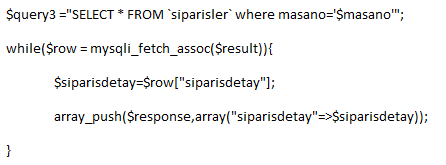
\includegraphics[scale=0.7]{c}
%Bu komutla resim dosyam�z� y�kl�yoruz.

\centering

\end{figure}
Sipari�ler tablosuna ula��ld���nda masa numaras�na g�re sipari� detay� �ekilir. 
\newpage
\subsection{Uygulama Ekran G�r�nt�leri}
Uygulamam 3 k�s�mdan olu�maktad�r. �lki men�, ikincisi mutfak ve ���nc�s� kasad�r.
\subsubsection{Men� Ekran�}
Uygulamaya girildi�inde ilk kar��m�za men� k�sm� ��kar. �ekil 10 'da men� ekran� g�r�lmektedir. Buradan istedi�imiz  kategoriden istenilen  �r�n se�ilerek �zet men�s�ne gelinir.
     \begin{figure}[H]
     \centering
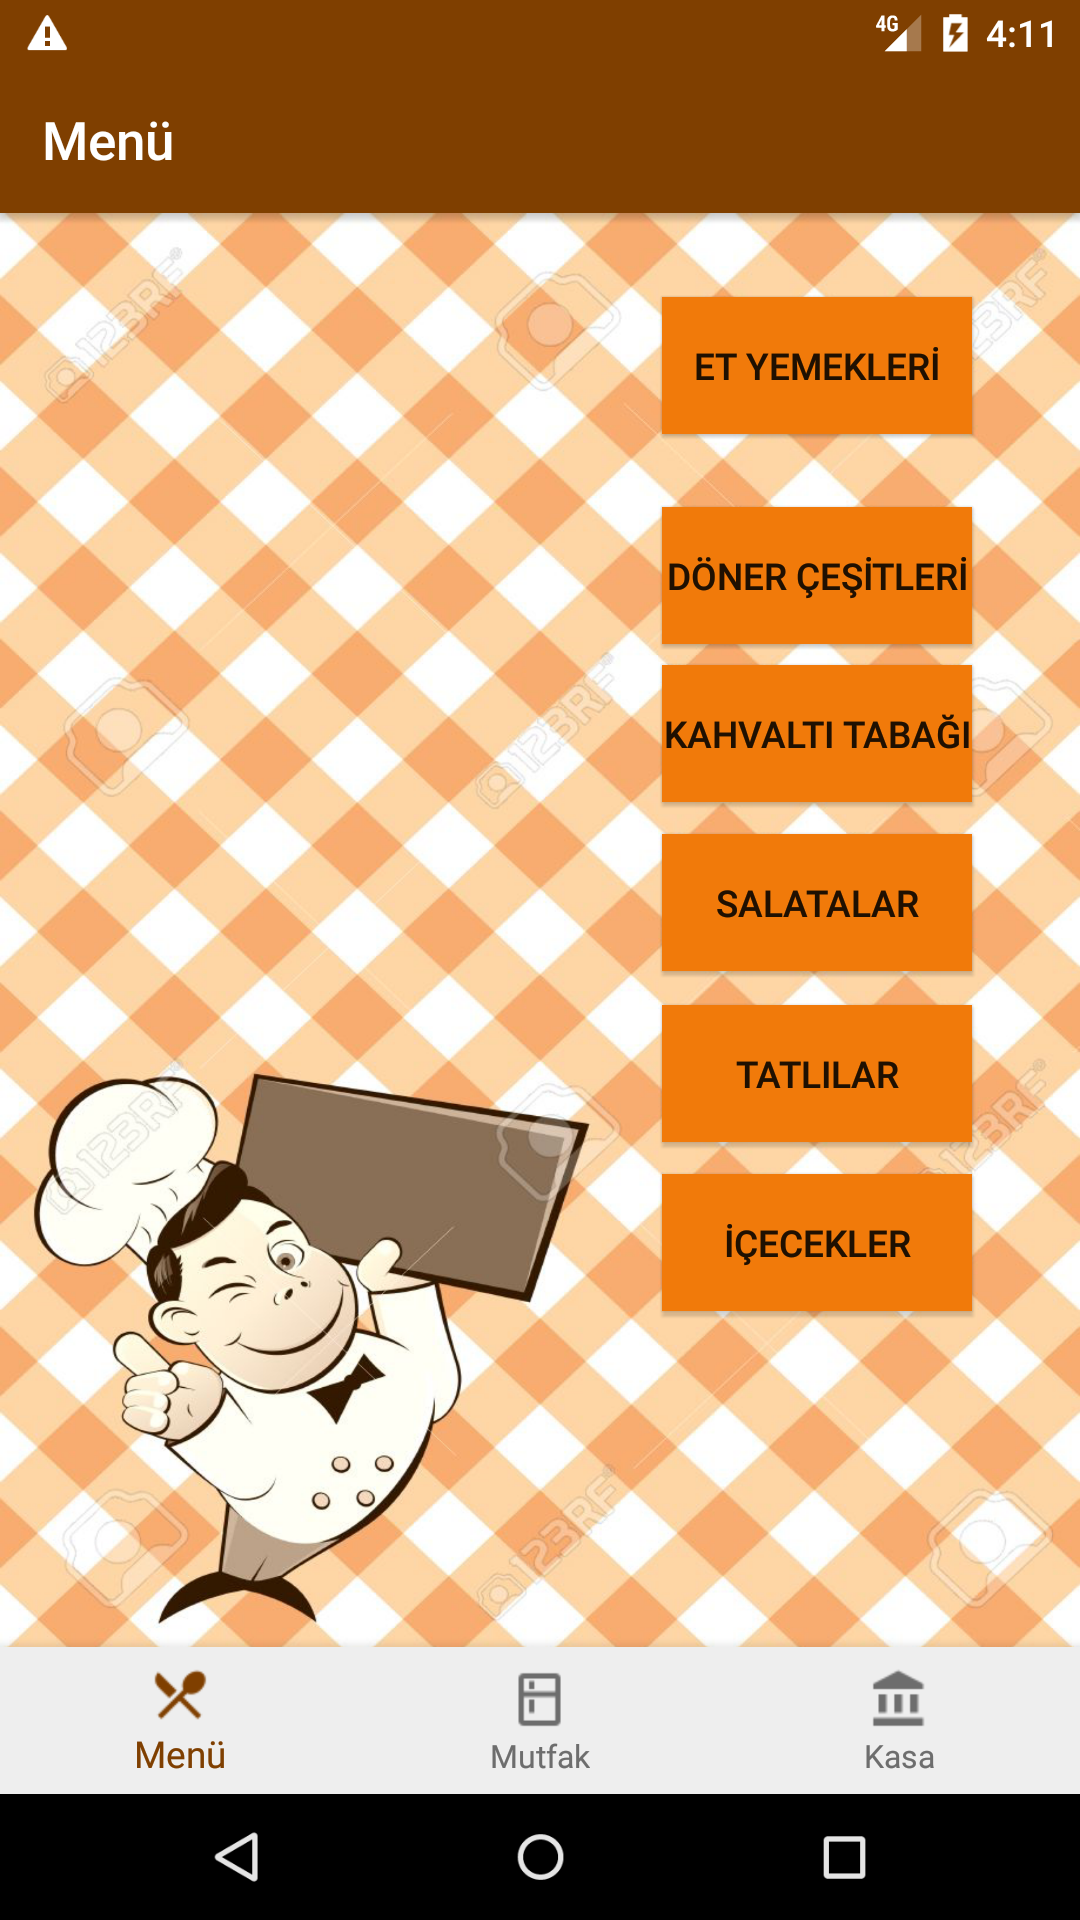
\includegraphics[scale=0.2]{menu}

\centering
�ekil 10:Men� Ekran�
\end{figure}
\subsubsection{�r�nler Ekran�}
Burada sipari�i devam ettirebilmek i�in devam butonu konuldu. Bu buton sayesinde ilk k�sma gelir. �stenilen �r�nler se�ilmeye devam edilir. �ekil 11'de g�r�lmektedir.

\begin{figure}[H]
     \centering
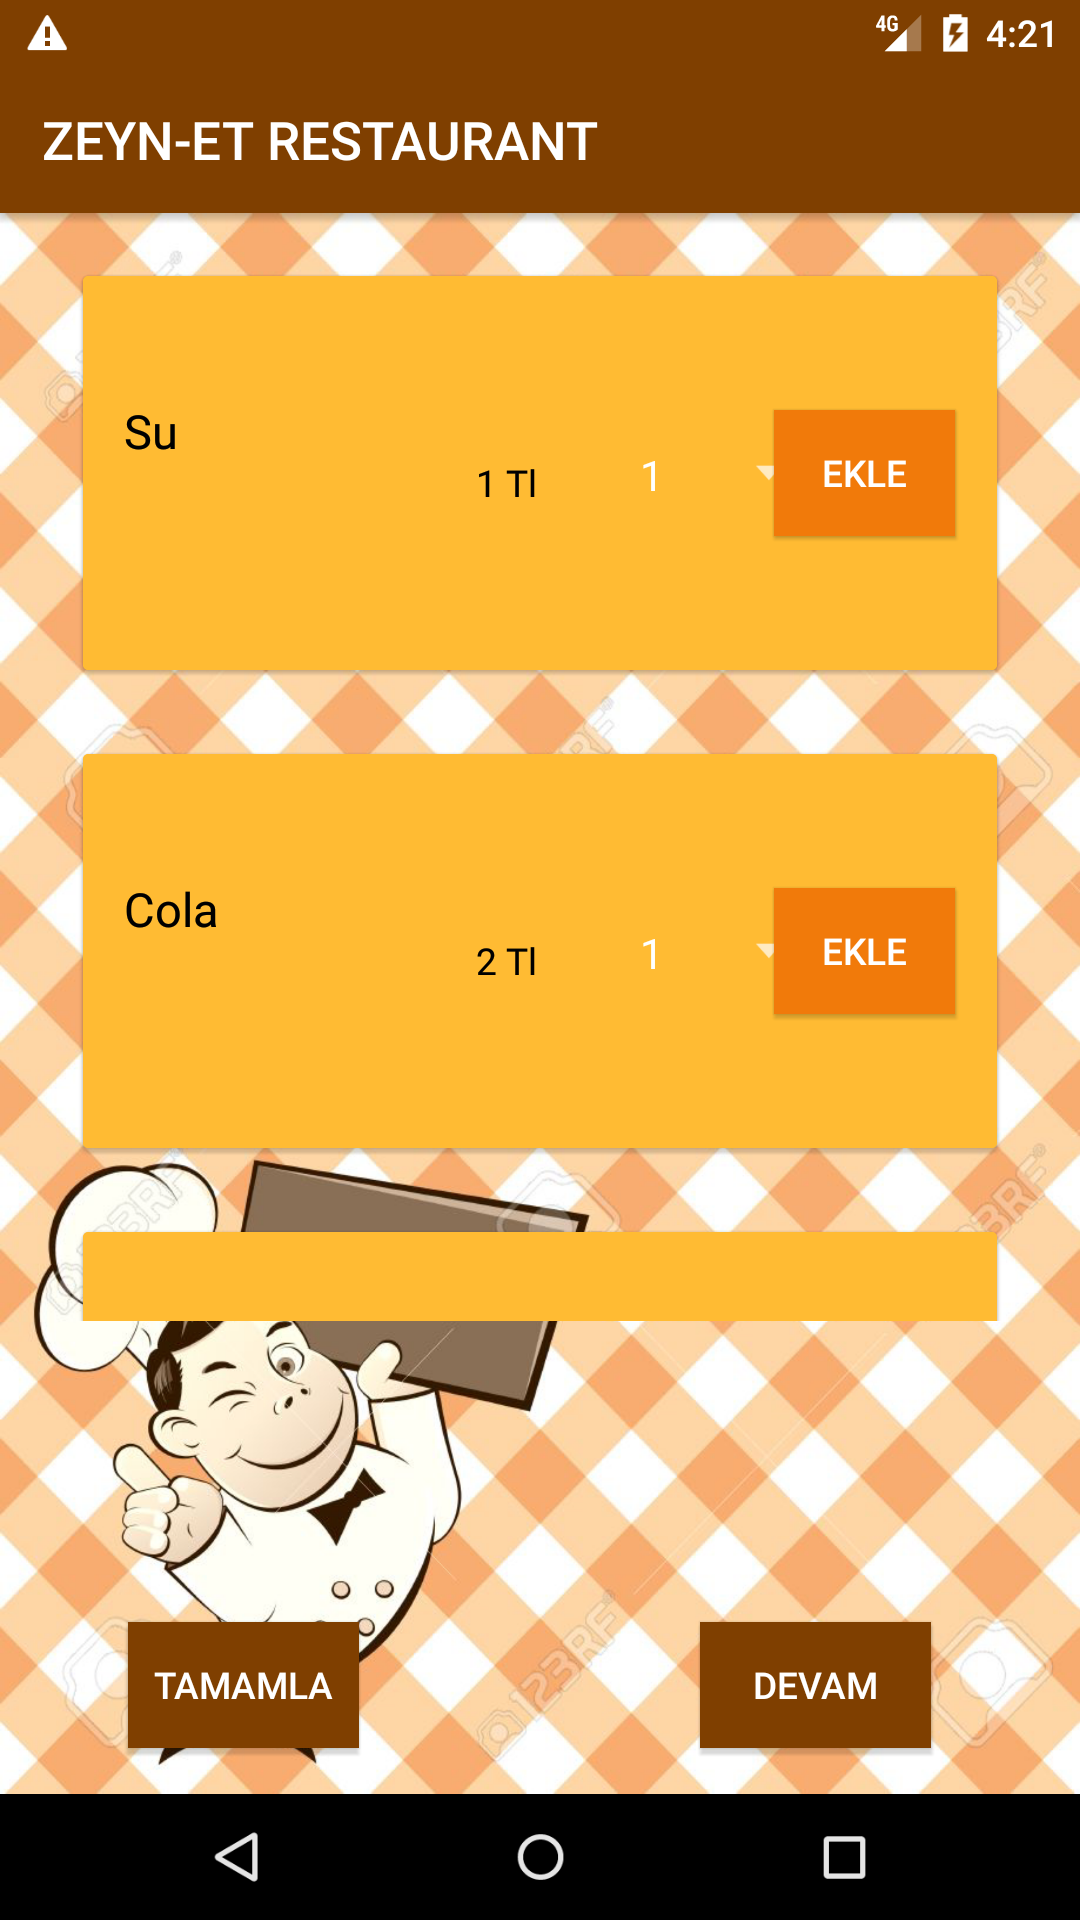
\includegraphics[scale=0.2]{menu1}

\centering
�ekil 11:�r�n Se�me
\end{figure}
\newpage
\subsubsection{Sipari� Tamamlama Ekran�}

M��teri sipari�lerini bitirdi�inde �r�n se�me k�sm�ndaki tamamla butonuna bast���nda sipari� tamamlama sayfas� gelir ve burada ne sipari� verildi�ini, toplam �denecek tutar� g�r�n�r. Ayr�yeten bu k�s�mda m��teriden masa numaras� bilgisinin girilmesi istenmektedir. Bu i�lemide ger�ekle�tiren m��teri i�in tek bir tu�a basmak yeterli olmu� olur art�k. Veritaban�na m��terinin sipari�leri kaydolur ve bu sipari�ler mutfak ve kasa k�sm�ndan giri� yapan personellere iletilmi� olunur.



Sipari�ler bitti�inde onaylan�l�r ve sipari�ler veritaban�ndaki sipari� tablosuna eklenir. �ekil 12'de g�r�lmektedir.

\begin{figure}[H]
     \centering
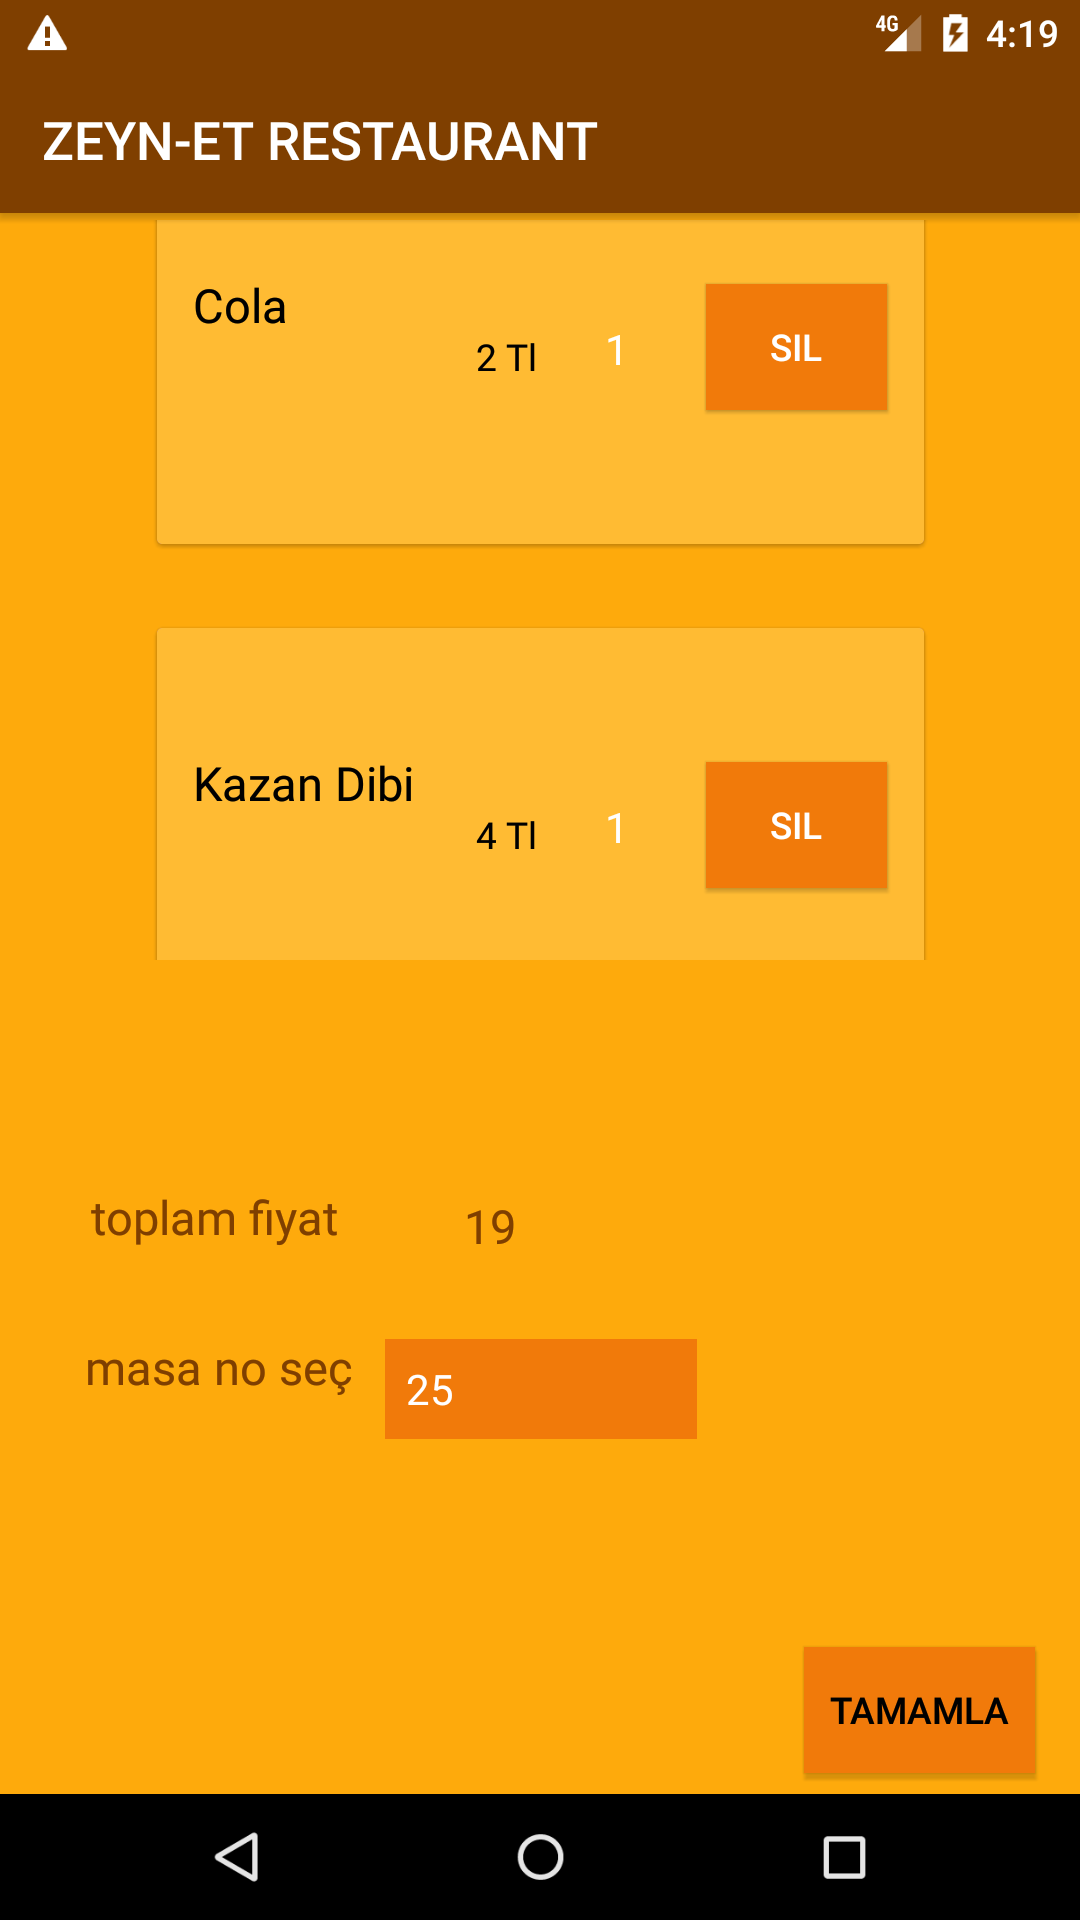
\includegraphics[scale=0.2]{menu2}

\centering
�ekil 12:Men� Sipari�i Tamamlama K�sm�
\end{figure}
\newpage
\subsubsection{Mutfak Giri� Ekran�}
Uygulaman�n ikinci k�sm� olan mutfak k�sm�na ge�ilecek olunursa, burada mutfak personelinin kullan�c� ad� ve �ifresini yazarak sisteme giri� yapmas�n� istenilir. Bu sayede personel harici bir ki�inin uygulaman�n bu alan�na eri�mesini engellenmi� olunur. �ekil 13'de g�sterilmektedir.
   \begin{figure}[H]
     \centering
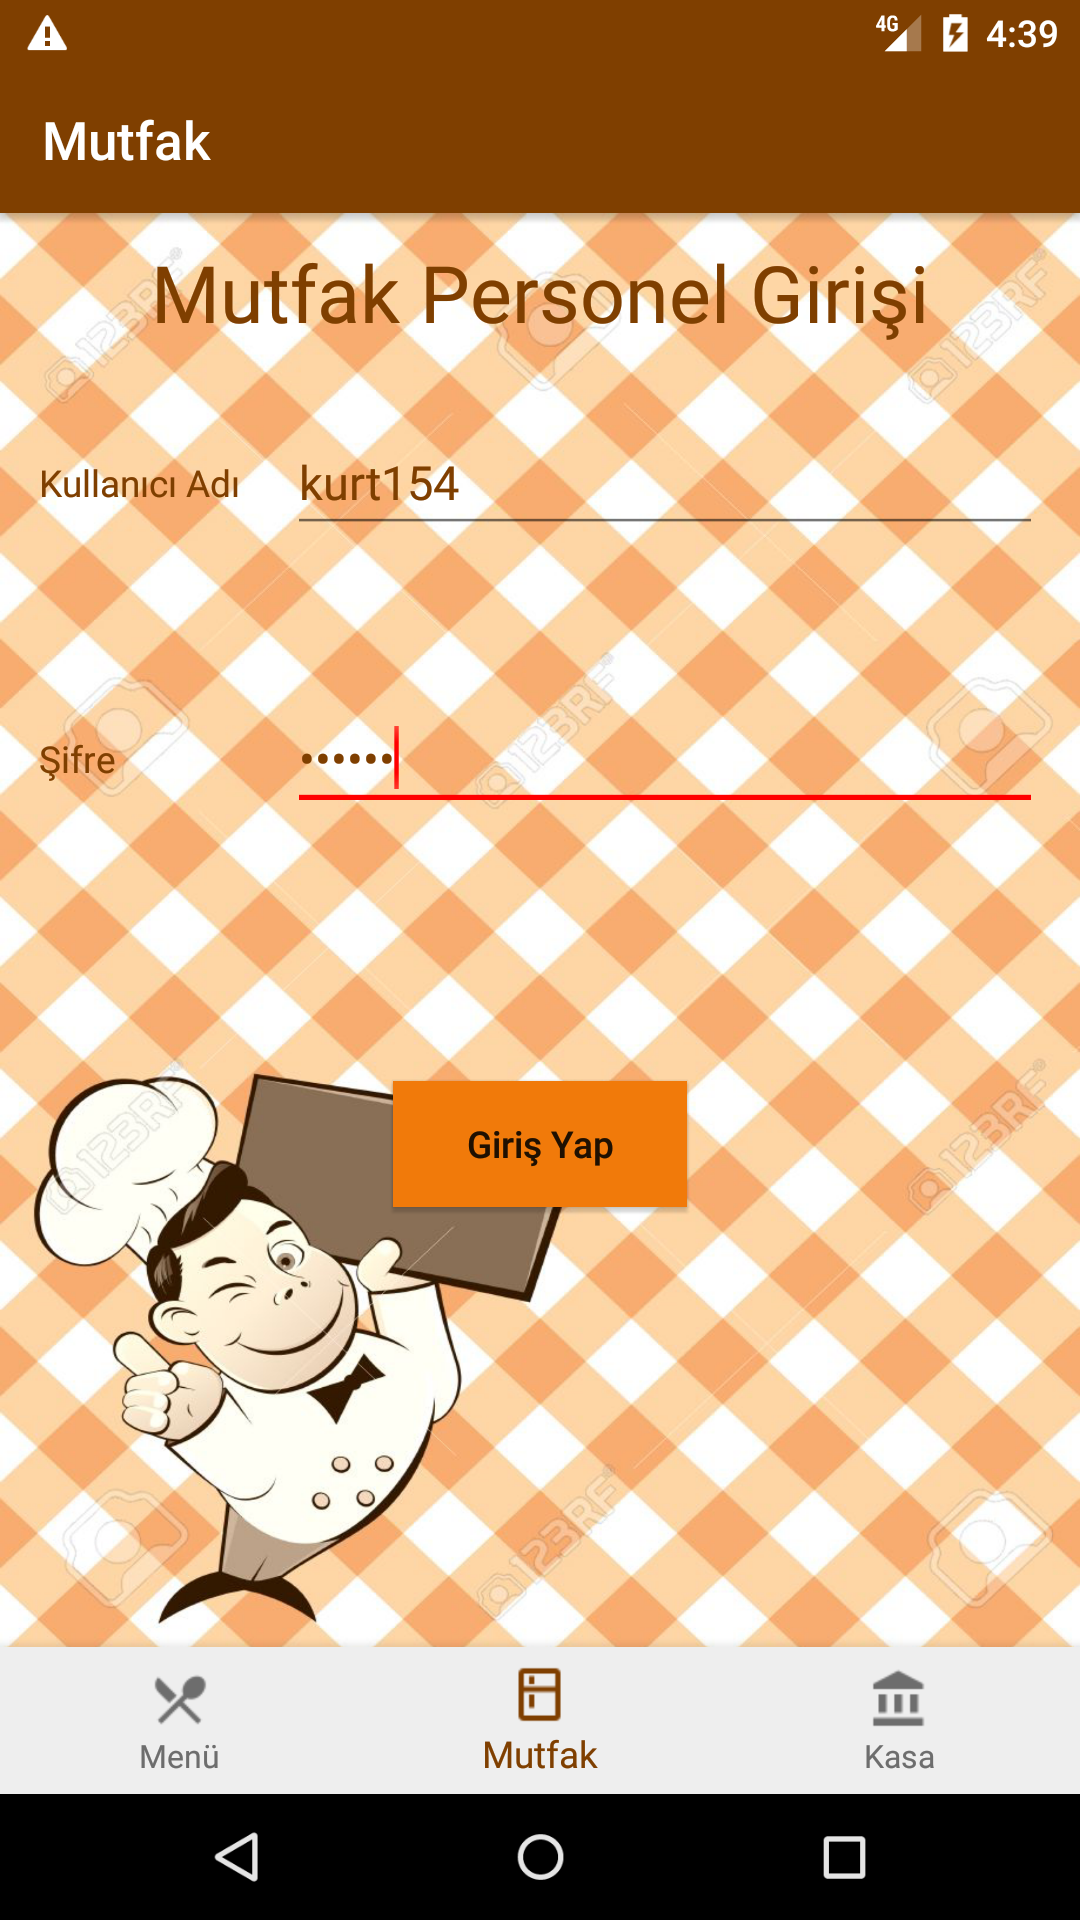
\includegraphics[scale=0.2]{mutfak}

\centering
�ekil 13:Mutfak Giri� Ekran�
\end{figure}
\newpage
\subsubsection{Masa Ekran�}
Personel giri� yapt�ktan sonra kar��s�na �ekil 14'deki ekran gelmektedir. Buradan  masalar�n isimlerinden hangi masan�n sipari�i ne o ��remi� olunur.
 \begin{figure}[H]
  \centering
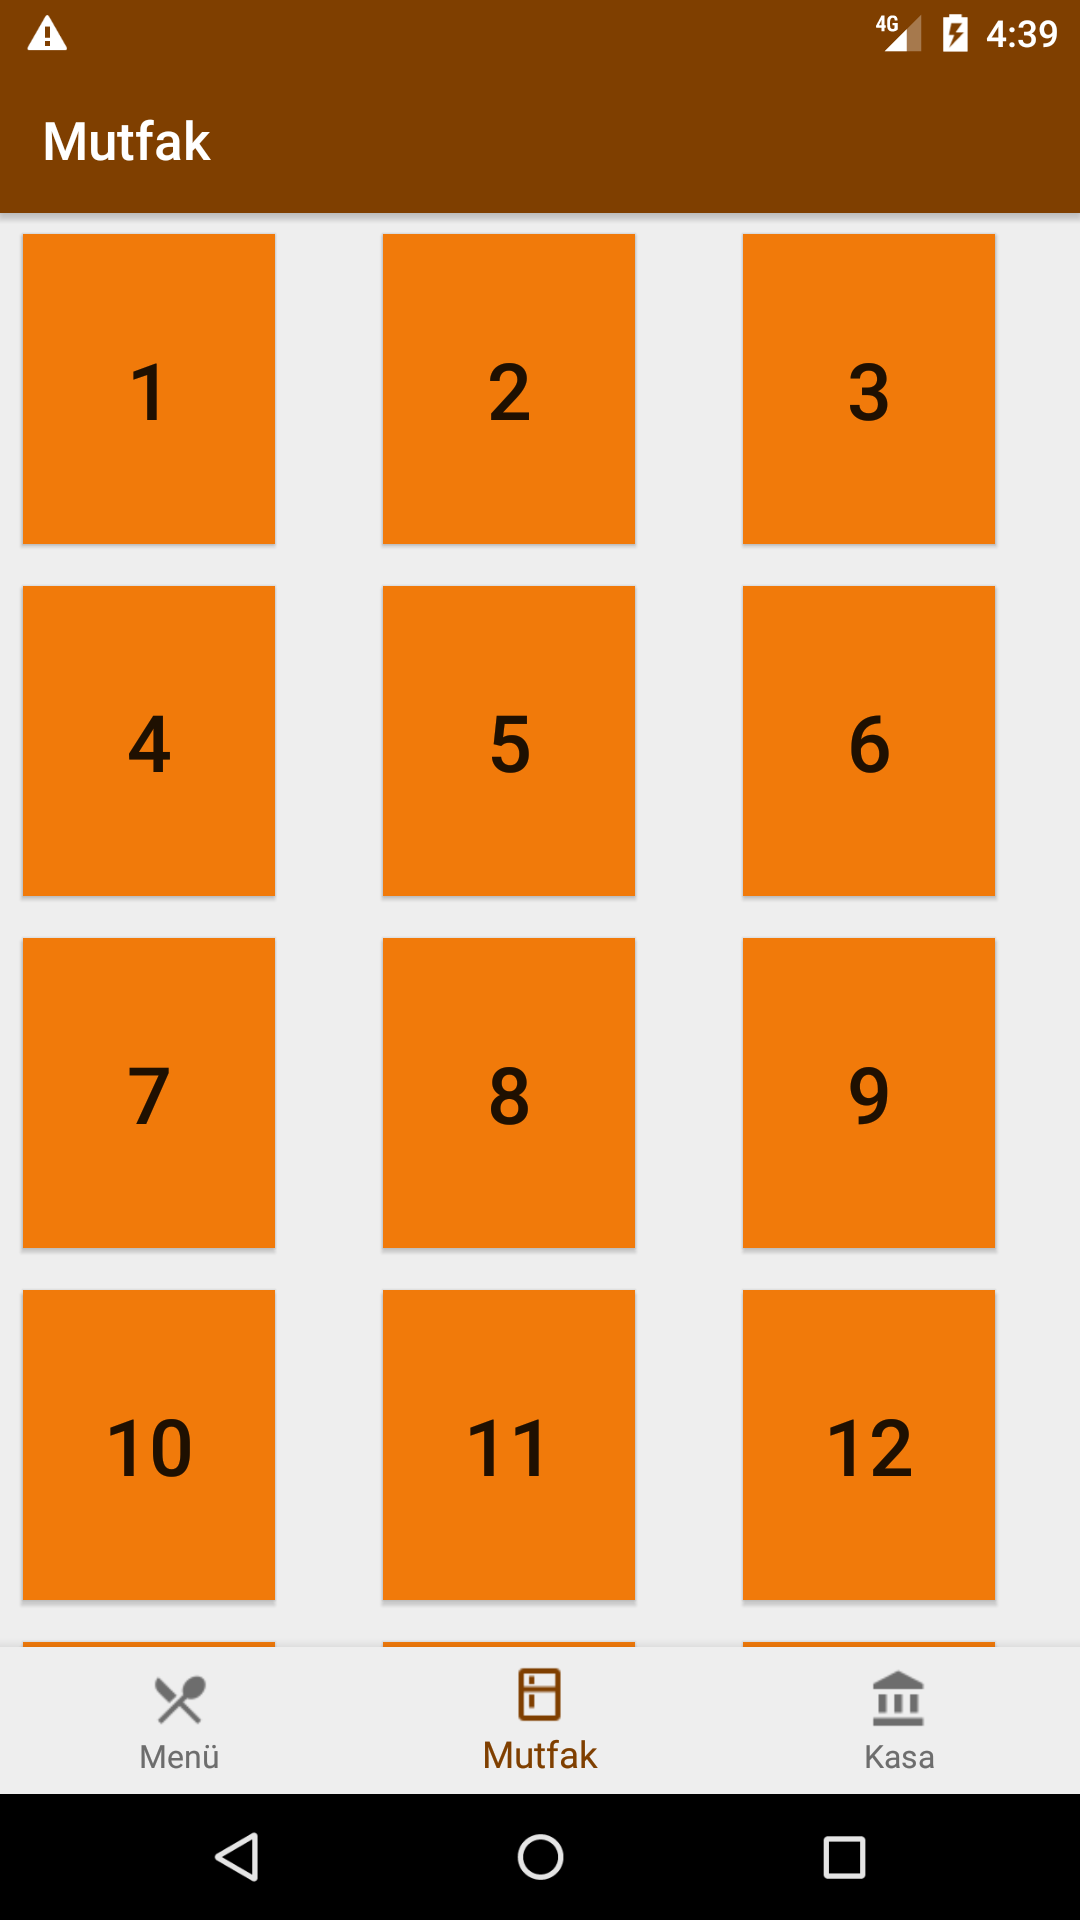
\includegraphics[scale=0.2]{mutfak1}

\centering
�ekil 14:Mutfak Masa Ekran�
\end{figure}
\newpage
\subsubsection{Masa Sipari� ekran�}
Giri� yapan personel herhangibir masaya t�klad���nda o masan�n sipari�leri g�r�lmektedir. �ekil 15'te ekran g�z�kmektedir.
\begin{figure}[H]
     \centering
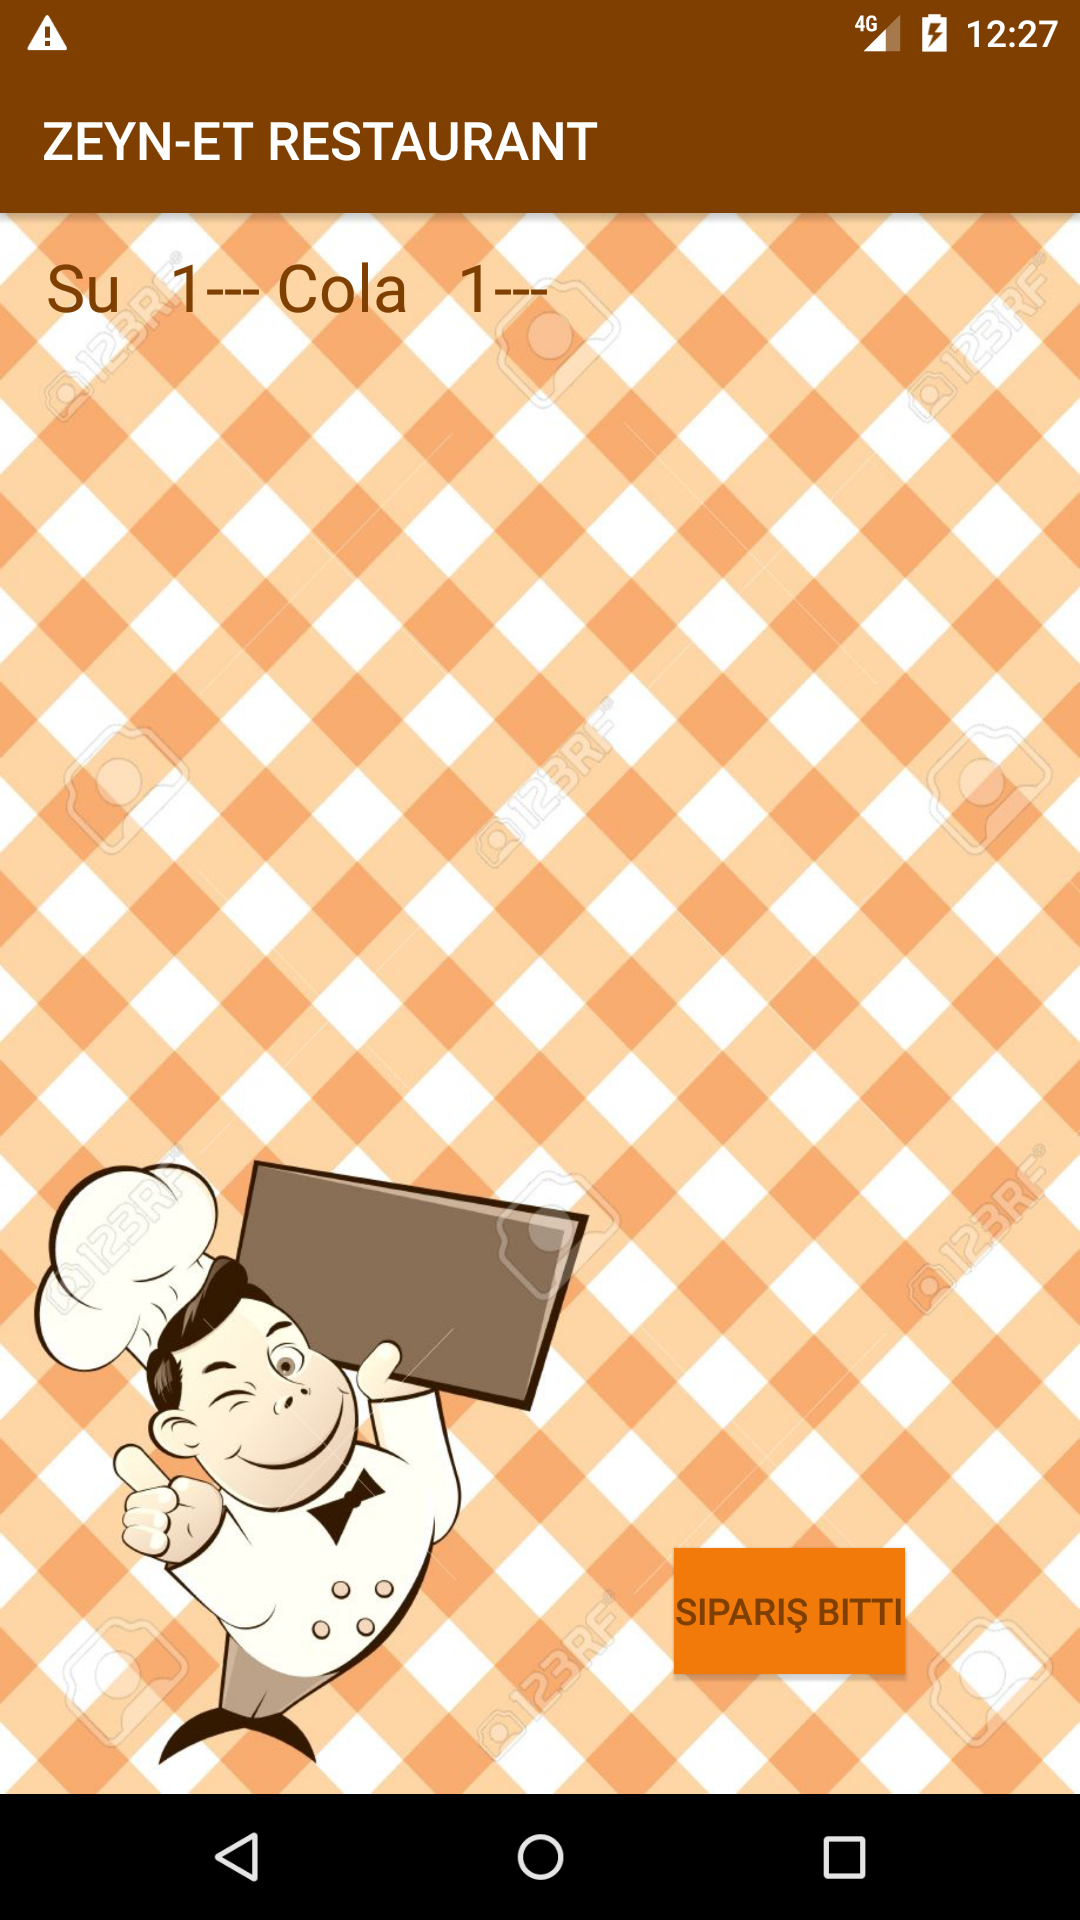
\includegraphics[scale=0.2]{mutfak2}

\centering
�ekil 15:Masa Sipari� Ekran�
\end{figure}

\subsubsection{Kasa Giri� Ekran�}
 Uygulaman�n ���nc� k�sm� olan kasa k�sm�na ge�ilecek olursa, burada kasa personelinin kullan�c� ad� ve �ifresini yazarak sisteme giri� yapmas�n� istenilir. Bu sayede personel harici bir ki�inin uygulaman�n bu alan�na eri�mesini engellenmi� olunur. Bu tasar�m mutfak k�sm�ndaki giri� ekran� ile ayn� oldu�u i�in ekan g�r�nt�s� konulmam��t�r.

\subsubsection{Masa Ekran�}
Personel giri� yapt�ktan sonra mutfak masa ekran�n�n ayn�s� gelmektedir.
\subsubsection{Kasa Hesap Ekran�}
Buradan  masalar�n isimlerinden hangi masan�n sipari�i ve hesab�n�n ne oldu�unu ��remi� olunur.
\begin{figure}[H]
\centering
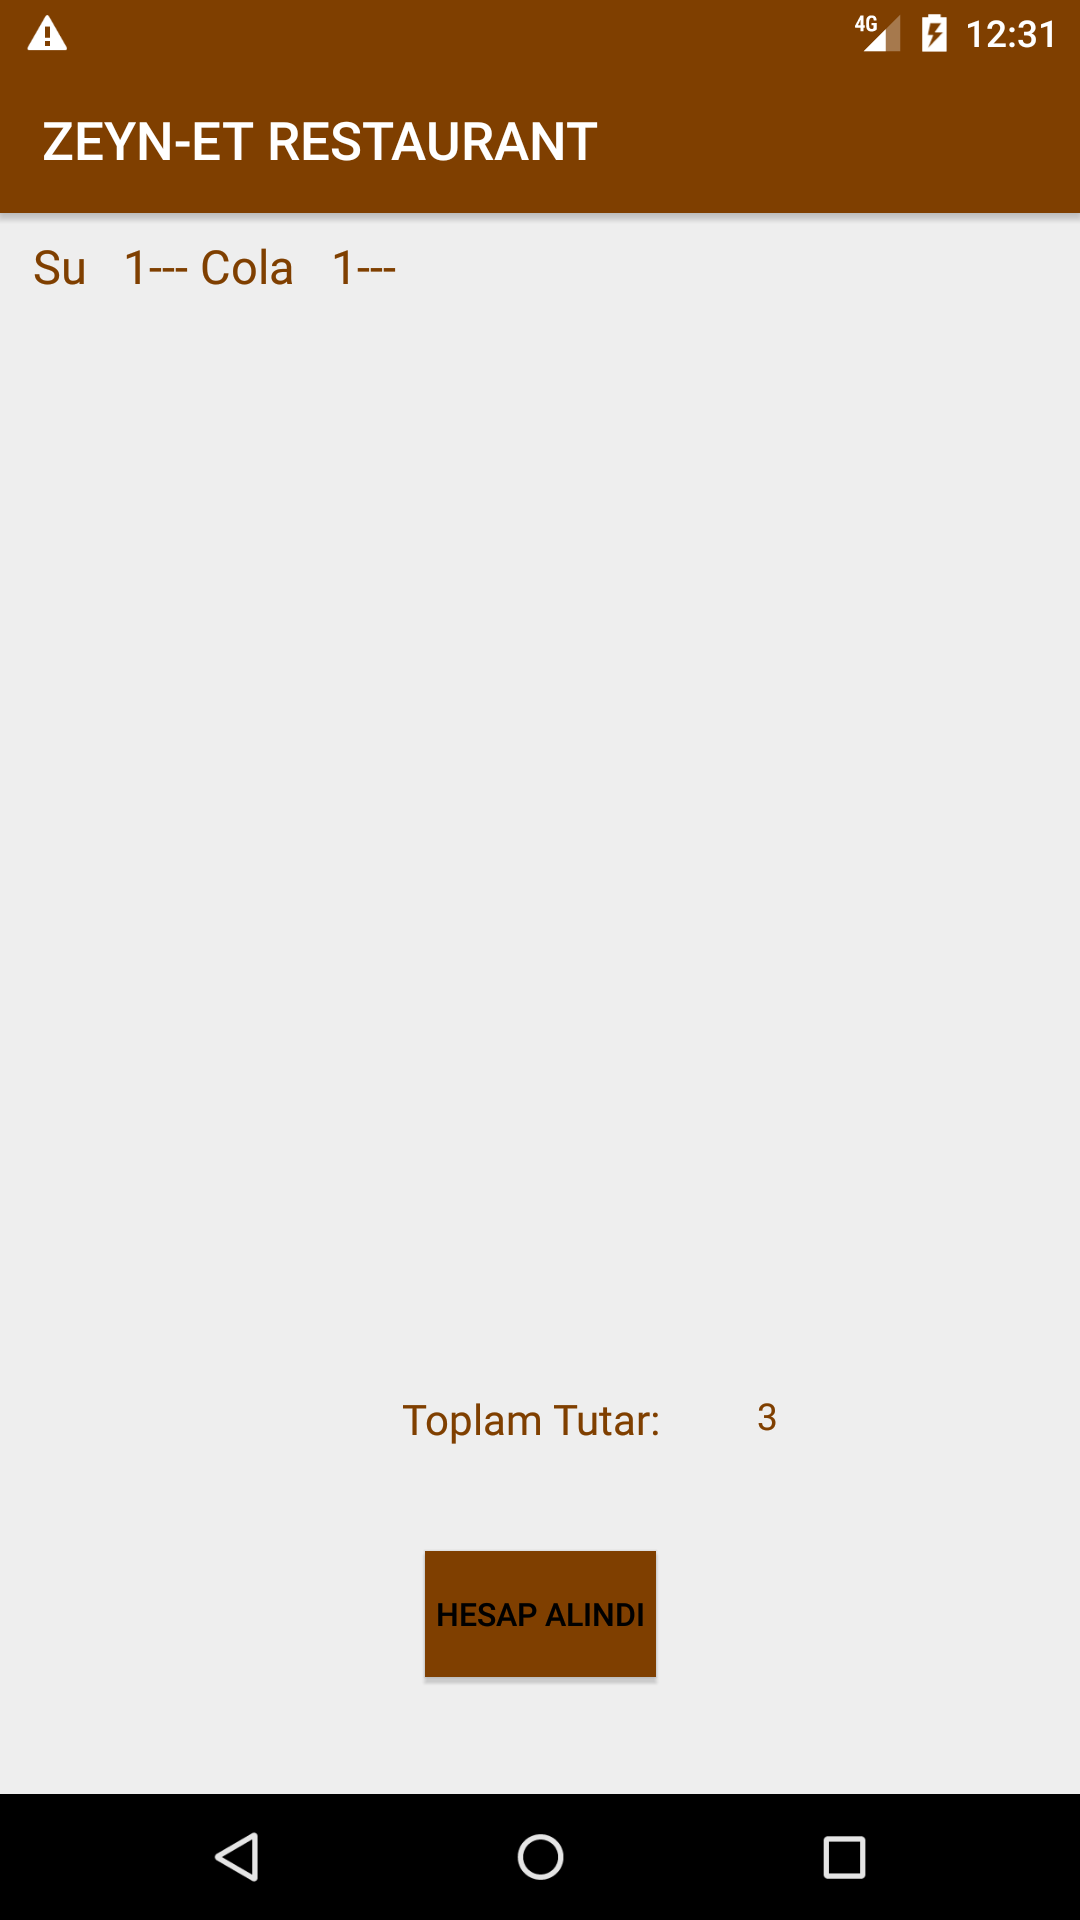
\includegraphics[scale=0.2]{kasa2}

\centering
�ekil 16:Kasa Hesap Ekran�
\end{figure}


 

\section{SONU�LAR VE �NER�LER}\label{S:4}
Bu projeyle birlikte restaurant imaj�nda yeni bir �ekile gidilmi�tir. Yap�lan bu proje kapsam�nda yeni nesil restaurantlar�n sipari� verme k�s�mlar� yeniden tasarland�. Tasar�m yap�l�rken daha g�n�m�z teknolojilerinden yararlan�lmaya �al���lm��t�r. G�n�m�zde yaz�l�m  bir �ok alanda kullan�lmakta ve insanlar�n hayat�n� kolayla�t�rmaktad�r.   Bu proje ile de yaz�l�m kullan�larak restaurantlar�n sipari� sistemi yeniden tasarland�. Bu sistemle restauranta gidildi�inde sipari� vermek i�in garsonu �a��rmaya veya beklemeye gerek kalmamaktad�r. Bunun yan�nda kasaya gitmeden sipari�lerin tutar� ��renilmi� olunur. �al��anlar a��s�ndan bak�lacak olunursa daha az g�� harcanm�� olunur. Ayr�yeten restaurant sahibi daha az �al��anla ayn� hizmeti m��terilerine sunabilmesiyle beraber daha az maliyet yam�� olur. 

Bu proje daha da geli�tirilebilir. Geli�tirilebilecek alanlar:
\begin{itemize}
\item Personele daha kolayl�k sa�lamak i�in masalara sipari� geldi�inde ye�il , sipari� haz�rland�ktan sonra silinince bir s�r� k�rm�z� kal�p tekrardan eski(uygulaman�n ba�taki buton rengi) haline d�nebilir.
\item M��terilerin restauranta gelmeden �nce rezervasyon yapabilmesi.
\item M��terilerin hesab� uygulama �zerinden kredi veya banka kart� ile �deyebilmesi.


\end{itemize}

\section{Ekler}


\subsection{Veritaban� ve Android Studio Aras�ndaki Ba�lant�y� Sa�layan Php Kodlar�}\label{ss:1}
\subsubsection{Personel Kayd� �ekme}\label{ss:1}
kayit.php i�erisinde  personel kayd�n� �ekmek i�in yaz�lm�� olan PHP kodlar� g�r�lmektedir.

<?php

function sorgu(\$mail){

	\$connect = mysqli\_connect("localhost","root","","restaurant");	
	\$query2 = "SELECT * FROM `personel` WHERE mail='".\$mail."'";
	
	\$result=mysqli\_query(\$connect, \$query2);
	
	\$sayac=0;
	
	while(\$row = mysqli\_fetch\_assoc(\$result)){
	
		if(\$mail==\$row["mail"])
		
			return false;//var demek
		else
		
		\$sayac=\$sayac+1;
				
	}
	
	if(\$sayac == 0)
	
		return true;
		
}


function sorgu2(\$mail,\$sifre){

	\$connect = mysqli\_connect("localhost","root","","restaurant");	
	
	\$query3 = "SELECT * FROM `personel` WHERE mail='".\$mail."'";
	
	\$result=mysqli\_query(\$connect, \$query3);
	
	\$sayac=0;
	
	while(\$row = mysqli\_fetch\_assoc(\$result)){
	
		if(\$sifre==\$row["sifre"])
		
			return false;//var demek
		else
		
		\$sayac=\$sayac+1;	//yok demek	
			
	}
	if(\$sayac == 1)
	
		return true;
		
}
\$connect = mysqli\_connect("localhost","root","","restaurant");	
	
\$mail=\$\_POST['mail'];

\$sifre=\$\_POST['sifre'];

\$response=array();

if(sorgu(\$mail)==false){


	if(sorgu2(\$mail,\$sifre)==false){
	
	\$code="dogru";
	
	\$message="giris tamam";
	
	array\_push(\$response,array("code"=>\$code,"message"=>\$message));
	
	echo json\_encode(\$response);
	

	}
	else if(sorgu2(\$mail,\$sifre)==true){
	
	\$code="yanlis";
	
	\$message="sifre yanlis";
	
	array\_push(\$response,array("code"=>\$code,"message"=>\$message));
	
	echo json\_encode(\$response);
	
	}	
	
}		

else if(sorgu(\$mail)==true)

{
	\$code="yanlis";
	
	\$message="boyle bir kullanici yok";
	
	array\_push(\$response,array("code"=>\$code,"message"=>\$message));
	
	echo json\_encode(\$response);
	
}

mysqli\_close(\$connect);

?>

\subsubsection{�r�n �ekme}\label{ss:1}
urun\_cek.php i�erisinde  m��terinin se�ti�i kategoriye g�re �r�nleri �ekmek i�in kullan�lm�� Php kodlar� g�r�lmektedir.

<?php


\$connect = mysqli\_connect("localhost","root","","restaurant");

	

\$kategori=\$\_POST['ktgr\_adi'];


\$query3 ="SELECT * FROM `urunler` where kategori\_adi='\$kategori'";



	\$result=mysqli\_query(\$connect, \$query3);
	
	\$response=array();
	
	while(\$row = mysqli\_fetch\_assoc(\$result)){
	
	\$urun\_id=\$row["urun\_id"];
	
	\$urun\_adi=\$row["urun\_adi"];
	
	\$kategori\_adi=\$row["kategori\_adi"];
	
	\$fiyat=\$row["fiyat"];
	
	array\_push(\$response,array("urun\_id"=>\$urun\_id,"urun\_adi"=>\$urun\_adi,
	
	"kategori\_adi"=>\$kategori\_adi,"fiyat"=>\$fiyat));
		

	}
	
	echo json\_encode(\$response);
	
	mysqli\_close(\$connect);

?>

\subsubsection{Fiyat �ekme}\label{ss:3}
fiyat\_cek.php i�erisinde  m��terinin se�ti�i kategoriye g�re �r�nlerin fiyatlar�n�n toplam�n� �ekmek i�in kullan�lm�� Php kodlar� g�r�lmektedir.

<?php
\$connect = mysqli\_connect("localhost","root","","restaurant");	

\$masano=\$\_POST['masano'];

\$query3 ="SELECT * FROM `siparisler` where masano='\$masano'";

\$result=mysqli\_query(\$connect, \$query3);

	\$response=array();
	
	
	while(\$row = mysqli\_fetch\_assoc(\$result)){
	
	\$siparisdetay=\$row["siparisdetay"];
	
	\$toplamtutar=\$row["toplamtutar"];
	
		array\_push(\$response,array("toplamtutar"=>\$toplamtutar,"siparisdetay"=>\$siparisdetay));
			

	}
	echo json\_encode(\$response);



	mysqli\_close(\$connect);


?>

\subsubsection{Sipari� �ekme}\label{ss:3}
siparis\_cek.php i�erisinde  m��terinin se�ti�i masa numaras�na g�re sadece personelin eri�ebildi�i k�sma ekler.Ve personel masa numaras�na t�klad��� zaman o masan�n sipari�lerini �ekmek i�in kullan�lan Php kodlar� g�sterilmektedir.
 
<?php

\$connect = mysqli\_connect("localhost","root","","restaurant");

	
\$masano=\$\_POST['masano'];

\$query3 ="SELECT * FROM `siparisler` where masano='\$masano'";

\$result=mysqli\_query(\$connect, \$query3);

	\$response=array();

while(\$row = mysqli\_fetch\_assoc(\$result)){

	\$siparisdetay=\$row["siparisdetay"];
	
	array\_push(\$response,array("siparisdetay"=>\$siparisdetay));	

	}
	
	echo json\_encode(\$response);



	mysqli\_close(\$connect);
	
?>


\subsubsection{Sipari� Ekleme}\label{ss:4}





siparis\_ekle.php i�erisinde  m��terinin se�ti�i kategoriye g�re �r�nleri al�p ve veritaban�na kaydeden Php kodlar� g�sterilmektedir.

<?php

\$connect = mysqli\_connect("localhost","root","","restaurant");	
\$masano=\$\_POST['masano'];

\$siparisdetay=\$\_POST['siparisdetay'];

\$toplamtutar=\$\_POST['toplamtutar'];



\$query = "INSERT INTO `siparisler` ( `masano`, `siparisdetay`, `toplamtutar`) VALUES ('".\$masano."','".\$siparisdetay."', '".\$toplamtutar."')";


\$response=array();


\$result=mysqli\_query(\$connect, \$query);


if(\$result){

	\$code="al�nd�";
	
	\$message="sipari�iniz al�nd� garsonu bekleyiniz";
	
	array\_push(\$response,array("code"=>\$code,"message"=>\$message));
	
	echo json\_encode(\$response);
	

}
else{
		\$code="al�namad�";
		
	\$message="sipari�iniz al�namad� garsonu �a��r�n�z";
	
	array\_push(\$response,array("code"=>\$code,"message"=>\$message));
	
	echo json\_encode(\$response);
	

}



?>
\subsection{Uygulama Tasar�m Kodlar�}\label{ss:2}
\subsubsection{Projenin Ana Sayfas� Tasar�m�}

<?xml version="1.0" encoding="utf-8"?>

<android.support.constraint.ConstraintLayout 

xmlns:android="http://schemas.android.com/apk/res/android"
    
    xmlns:app="http://schemas.android.com/apk/res-auto"
    
    xmlns:tools="http://schemas.android.com/tools"
    
    android:id="@+id/container"
    
    android:layout\_width="match\_parent"
    
    android:layout\_height="match\_parent"    
    
    tools:context="com.example.zeynep.bottombar.Activitys.MainActivity">

    
    <android.support.design.widget.BottomNavigationView
        
        android:id="@+id/navigation"
        
        android:layout\_width="0dp"
        
        android:layout\_height="wrap\_content"
        
        android:layout\_marginEnd="0dp"
        
        android:layout\_marginStart="0dp"
        
        android:background="?android:attr/windowBackground"
        
        app:layout\_constraintBottom\_toBottomOf="parent"
        
        app:layout\_constraintLeft\_toLeftOf="parent"
        
        app:layout\_constraintRight\_toRightOf="parent"
        
        app:menu="@menu/navigation" />

    <FrameLayout
    
        android:id="@+id/fram"
        android:layout\_width="match\_parent"
        
        android:layout\_height="match\_parent"
        
        android:layout\_marginBottom="55dp"
        
        app:layout\_constraintBottom\_toBottomOf="parent"
        
        app:layout\_constraintEnd\_toEndOf="parent"
        
        app:layout\_constraintStart\_toStartOf="parent"
        
        app:layout\_constraintTop\_toTopOf="parent"
        
        tools:ignore="MissingConstraints" 
        
        />


</android.support.constraint.ConstraintLayout>

\subsubsection{Men� Sayfas� Tasar�m Kodlar�}
<?xml version="1.0" encoding="utf-8"?>

<FrameLayout xmlns:android="http://schemas.android.com/apk/res/android"

    xmlns:app="http://schemas.android.com/apk/res-auto"
    
    xmlns:tools="http://schemas.android.com/tools"
    
    android:id="@+id/framelayout"
    
    android:layout\_width="match\_parent"
    android:layout\_height="match\_parent"
    
    tools:context="com.example.zeynep.bottombar.Fragments.FragmentOne"

    android:orientation="vertical"
    
    android:background="@drawable/r4">


        <android.support.constraint.ConstraintLayout
            
            android:layout\_width="match\_parent"
            
            android:layout\_height="match\_parent"
            
            android:visibility="visible">


                <Button
                
                    android:id="@+id/spinner2"
                    
                    android:layout\_width="118dp"
                    
                    android:layout\_height="52dp"
                    
                    android:layout\_marginBottom="8dp"
                    
                    android:layout\_marginEnd="8dp"
                    
                    android:layout\_marginStart="8dp"
                    
                    android:layout\_marginTop="8dp"
                    
                    android:background="?android:attr/colorActivatedHighlight"
                    
                    android:gravity="center"
                    
                    android:text="ET YEMEKLER�"
                    
                    app:layout\_constraintBottom\_toBottomOf="parent"
                    
                    app:layout\_constraintEnd\_toEndOf="parent"
                    
                    app:layout\_constraintHorizontal\_bias="0.88"
                    
                    app:layout\_constraintStart\_toStartOf="parent"
                    
                    app:layout\_constraintTop\_toTopOf="parent"
                    
                    app:layout\_constraintVertical\_bias="0.050000012" />
                    

                <Button
                
                    android:id="@+id/d�ner"
                    
                    android:layout\_width="118dp"
                    
                    android:layout\_height="52dp"
                    
                    android:layout\_marginBottom="8dp"
                    
                    android:layout\_marginEnd="8dp"                                        
                    
                    android:layout\_marginStart="8dp"
                    
                    android:layout\_marginTop="8dp"
                    
                    android:background="?android:attr/colorActivatedHighlight"
                    
                    android:gravity="center"
                    
                    android:text="D�NER �E��TLER�"
                    
                    app:layout\_constraintBottom\_toBottomOf="parent"
                    
                    app:layout\_constraintEnd\_toEndOf="parent"
                    
                    app:layout\_constraintHorizontal\_bias="0.88"
                    
                    app:layout\_constraintStart\_toStartOf="parent"
                    
                    app:layout\_constraintTop\_toBottomOf="@+id/spinner2"
                    
                    app:layout\_constraintVertical\_bias="0.050000012" />
                    

                <Button
                
                    android:id="@+id/tatli"
                    
                    android:layout\_width="118dp"                                                            
                    
                    android:layout\_height="52dp"
                    
                    android:layout\_marginBottom="100dp"
                    
                    android:layout\_marginEnd="8dp"
                    
                    android:layout\_marginStart="8dp"
                    
                    android:layout\_marginTop="8dp"
                    
                    android:background="?android:attr/colorActivatedHighlight"
                    
                    android:gravity="center"
                    
                    android:text="TATLILAR"
                    
                    app:layout\_constraintBottom\_toBottomOf="parent"
                    
                    app:layout \_constraintEnd\_toEndOf="parent"
                    
                    app:layout\_constraintHorizontal\_bias="0.88"
                    
                    app:layout\_constraintStart\_toStartOf="parent"
                    
                    app:layout\_constraintTop\_toBottomOf="@+id/salata"
                    
                    app:layout\_constraintVertical\_bias="0.050000012" />
                    

                <Button
                
                    android:id="@+id/salata"
                    
                    android:layout\_width="118dp"
                    
                    android:layout\_height="52dp"
                    
                    android:layout\_marginBottom="180dp"
                    
                    android:layout\_marginEnd="8dp"
                    
                    android:layout\_marginStart="8dp"
                    
                    android:layout\_marginTop="8dp"
                    
                    android:background="?android:attr/colorActivatedHighlight"
                    
                    android:gravity="center"
                    
                    android:text="SALATALAR"
                    
                    app:layout\_constraintBottom\_toBottomOf="parent"
                    
                    app:layout\_constraintEnd\_toEndOf="parent"
                    
                    app:layout\_constraintHorizontal\_bias="0.88"                                        
                    
                    app:layout\_constraintStart\_toStartOf="parent"
                    
                    app:layout\_constraintTop\_toBottomOf="@+id/kahvalti"
                    
                    app:layout\_constraintVertical\_bias="0.050000012" />
                    

                <Button
                
                    android:id="@+id/kahvalti"
                    
                    android:layout\_width="118dp"
                    
                    android:layout\_height="52dp"
                    
                    android:layout\_marginBottom="264dp"
                    
                    android:layout\_marginEnd="8dp"
                    
                    android:layout\_marginStart="8dp"
                    
                    android:layout\_marginTop="8dp"
                    
                    android:background="?android:attr/colorActivatedHighlight"
                    
                    android:gravity="center"
                    
                    android:text="KAHVALTI TABA�I"
                
                    app:layout\_constraintBottom\_toBottomOf="parent"
                    
                    app:layout\_constraintEnd\_toEndOf="parent"
                    
                    app:layout\_constraintHorizontal\_bias="0.88"
                    
                    app:layout\_constraintStart\_toStartOf="parent"
                    
                    app:layout\_constraintTop\_toBottomOf="@+id/d�ner"
                    
                    app:layout\_constraintVertical\_bias="0.0" />
                    

                <Button
                
                    android:id="@+id/icecekler"
                    
                    android:layout\_width="118dp"
                    
                    android:layout\_height="52dp"
                    
                    android:layout\_marginBottom="48dp"
                    
                    android:layout\_marginEnd="8dp"
                    
                    android:layout\_marginStart="8dp"
                    
                    android:layout\_marginTop="8dp"
                    
                    android:background="?android:attr/colorActivatedHighlight"
                    
                    android:gravity="center"
                    
                    android:text="��ECEKLER"
                    
                    app:layout\_constraintBottom\_toBottomOf="parent"
                    
                    app:layout\_constraintEnd\_toEndOf="parent"
                    
                    app:layout\_constraintHorizontal\_bias="0.88"
                    
                    app:layout\_constraintStart\_toStartOf="parent"
                    
                    app:layout\_constraintTop\_toBottomOf="@+id/tatli"
                    
                    app:layout\_constraintVertical\_bias="0.050000012" />
                    

        </android.support.constraint.ConstraintLayout>



</FrameLayout>

\subsubsection{�r�n  Sayfas� Tasar�m Kodlar�}

<?xml version="1.0" encoding="utf-8"?>

<android.support.v7.widget.CardView 

xmlns:android="http://schemas.android.com/apk/res/android"
    
    xmlns:app="http://schemas.android.com/apk/res-auto"
    
    xmlns:tools="http://schemas.android.com/tools"
    
    android:layout\_width="match\_parent"
    
    android:layout\_height="150dp"
    
    android:layout\_margin="16dp"
    
    app:cardBackgroundColor="@android:color/holo\_orange\_light">

    <android.support.constraint.ConstraintLayout
        android:layout\_width="match\_parent"
        
        android:layout\_height="match\_parent"
        
        android:background="\#a0522d"
        
        android:backgroundTint="@android:color/holo\_orange\_light">

        <TextView
        
            android:id="@+id/urun\_adi"
            
            android:layout\_width="125dp"
            
            android:layout\_height="57dp"
            
            android:layout\_marginBottom="8dp"
            
            android:layout\_marginEnd="8dp"
            
            android:layout\_marginStart="8dp"
            
            android:layout\_marginTop="8dp"
            
            android:text="�r�n ad�"
            
            android:textColor="\#000"
            
            android:textSize="18sp"
            
            app:layout\_constraintBottom\_toBottomOf="parent"
            
            app:layout\_constraintEnd\_toEndOf="parent"
            
            app:layout\_constraintHorizontal\_bias="0.037"
            
            app:layout\_constraintStart\_toStartOf="parent"
            
            app:layout\_constraintTop\_toTopOf="parent"
            
            app:layout\_constraintVertical\_bias="0.506" />
            

        <Spinner
        
            android:id="@+id/spinner"
            
            android:layout\_width="67dp"
            
            android:layout\_height="21dp"
            
            android:layout\_marginBottom="8dp"
            
            android:layout\_marginEnd="8dp"
            
            android:layout\_marginStart="8dp"
            
            android:layout\_marginTop="8dp"
            
            app:layout\_constraintBottom\_toBottomOf="parent"
            
            app:layout\_constraintEnd\_toEndOf="parent"
            
            app:layout\_constraintHorizontal\_bias="0.74"
            
            app:layout\_constraintStart\_toStartOf="parent"
            
            app:layout\_constraintTop\_toTopOf="parent" />
            

        <TextView
        
            android:id="@+id/fiyat"
            
            android:layout\_width="49dp"
            
            android:layout\_height="19dp"
            
            android:layout\_marginEnd="8dp"
            
            android:layout\_marginStart="8dp"
            
            android:layout\_marginTop="4dp"
            
            android:text="fiyat"
            
            android:textColor="@android:color/background\_dark"
            
            app:layout\_constraintEnd\_toEndOf="parent"
            
            app:layout\_constraintStart\_toStartOf="parent"
            
            app:layout\_constraintTop\_toTopOf="@+id/spinner" />
            

        <Button
        
            android:id="@+id/ekle"
            
            android:layout\_width="69dp"
            
            android:layout\_height="48dp"
            
            android:layout\_marginBottom="8dp"
            
            android:layout\_marginEnd="8dp"
            
            android:layout\_marginStart="8dp"
            
            android:layout\_marginTop="8dp"
            
            android:background="?android:attr/colorActivatedHighlight"
            
            android:backgroundTint="?android:attr/colorMultiSelectHighlight"
            
            android:text="EKLE"
            
            app:layout\_constraintBottom\_toBottomOf="parent"
            
            app:layout\_constraintEnd\_toEndOf="parent"
            
            app:layout\_constraintHorizontal\_bias="0.97"
            
            app:layout\_constraintStart\_toStartOf="parent"
            
            app:layout\_constraintTop\_toTopOf="parent"
            
            tools:ignore="OnClick" />
            
    </android.support.constraint.ConstraintLayout>


</android.support.v7.widget.CardView>




\subsubsection{�zet Sayfas� Tasar�m Kodlar�}
<?xml version="1.0" encoding="utf-8"?>

<android.support.constraint.ConstraintLayout 

xmlns:android="http://schemas.android.com/apk/res/android"

    xmlns:app="http://schemas.android.com/apk/res-auto"
    
    xmlns:tools="http://schemas.android.com/tools"
    
    android:layout\_width="match\_parent"
    
    android:layout\_height="match\_parent"
    
    android:background="@android:color/holo\_orange\_light"
    
    android:backgroundTint="?android:attr/colorPressedHighlight"
    
    tools:context="com.example.zeynep.bottombar.Activitys.OzetHesap">

    
    <android.support.v7.widget.RecyclerView
        android:id="@+id/rccyl"
        
        android:layout\_width="324dp"
        
        android:layout\_height="282dp"
        
        app:layout\_constraintBottom\_toBottomOf="parent"
        
        app:layout\_constraintEnd\_toEndOf="parent"
        
        app:layout\_constraintStart\_toStartOf="parent"
        
        app:layout\_constraintTop\_toTopOf="parent"
        
        app:layout\_constraintVertical\_bias="0.008" />
        

    <Button
    
        android:id="@+id/oksiparis"
        
        android:layout\_width="wrap\_content"
        
        android:layout\_height="wrap\_content"
        
        android:layout\_marginBottom="8dp"
        
        android:layout\_marginEnd="8dp"
        
        android:layout\_marginStart="8dp"
        
        android:layout\_marginTop="8dp"
        
        android:background="?android:attr/colorActivatedHighlight"
        
        android:text="tamamla"
        
        android:textColor="?android:attr/colorForeground"
        
        app:layout\_constraintBottom\_toBottomOf="parent"
        
        app:layout\_constraintEnd\_toEndOf="parent"
        
        app:layout\_constraintHorizontal\_bias="0.97"
        
        app:layout\_constraintStart\_toStartOf="parent"
        
        app:layout\_constraintTop\_toTopOf="parent"
        
        app:layout\_constraintVertical\_bias="1.0" />
        

    <TextView
    
        android:id="@+id/textView2"
        
        android:layout\_width="wrap\_content"
        
        android:layout\_height="wrap\_content"
        
        android:layout\_marginBottom="8dp"
        
        android:layout\_marginEnd="8dp"
        
        android:layout\_marginStart="8dp"
        
        android:layout\_marginTop="8dp"
        
        android:text="toplam fiyat"
        
        android:textColor="@color/colorPrimaryDark"
        
        android:textColorLink="@color/colorPrimaryDark"
        
        android:textSize="18sp"
        
        app:layout\_constraintBottom\_toBottomOf="parent"
        
        app:layout\_constraintEnd\_toEndOf="parent"
        
        app:layout\_constraintHorizontal\_bias="0.088"
        
        app:layout\_constraintStart\_toStartOf="parent"
        
        app:layout\_constraintTop\_toTopOf="parent"
        
        app:layout\_constraintVertical\_bias="0.644" />
        

    <TextView
    
        android:id="@+id/ozethesap"
        
        android:layout\_width="83dp"
        
        android:layout\_height="21dp"
        
        android:layout\_marginBottom="8dp"
        
        android:layout\_marginEnd="8dp"
        
        android:layout\_marginStart="8dp"
        
        android:layout\_marginTop="8dp"
        
        android:text="TextView"
        
        android:textColor="@color/colorPrimaryDark"
        
        android:textColorHighlight="@color/colorPrimaryDark"
        
        android:textColorLink="@color/colorPrimaryDark"
        
        android:textSize="18sp"
        
        app:layout\_constraintBottom\_toBottomOf="parent"
        
        app:layout\_constraintEnd\_toEndOf="parent"
        
        app:layout\_constraintHorizontal\_bias="0.54"
        
        app:layout\_constraintStart\_toStartOf="parent"
        
        app:layout\_constraintTop\_toTopOf="parent"
        
        app:layout\_constraintVertical\_bias="0.647" />
        

    <Spinner
    
        android:id="@+id/spinner2"
        
        android:layout\_width="119dp"
        
        android:layout\_height="38dp"
        
        android:layout\_marginBottom="8dp"
        
        android:layout\_marginEnd="8dp"
        
        android:layout\_marginStart="8dp"
        
        android:layout\_marginTop="8dp"
        
        android:background="?android:attr/colorMultiSelectHighlight"
        
        android:popupBackground="@android:color/holo\_orange\_light"
        
        app:layout\_constraintBottom\_toBottomOf="parent"
        
        app:layout\_constraintEnd\_toEndOf="parent"
        
        app:layout\_constraintHorizontal\_bias="0.502"
        
        app:layout\_constraintStart\_toStartOf="parent"
        
        app:layout\_constraintTop\_toTopOf="parent"
        
        app:layout\_constraintVertical\_bias="0.768" />
        

    <TextView
    
        android:id="@+id/textView4"
        
        android:layout\_width="wrap\_content"        
        
        android:layout\_height="wrap\_content"
        
        android:layout\_marginBottom="8dp"
        
        android:layout\_marginEnd="8dp"
        
        android:layout\_marginStart="8dp"
        
        android:layout\_marginTop="8dp"
        
        android:text="masa no se�"
        
        android:textColor="@color/colorPrimaryDark"
        
        android:textColorLink="@color/colorPrimaryDark"
        
        android:textSize="18sp"
        
        app:layout\_constraintBottom\_toBottomOf="parent"
        
        app:layout\_constraintEnd\_toEndOf="parent"
        
        app:layout\_constraintHorizontal\_bias="0.083"
        
        app:layout\_constraintStart\_toStartOf="parent"
        
        app:layout\_constraintTop\_toTopOf="parent"
        
        app:layout\_constraintVertical\_bias="0.746" />
        
</android.support.constraint.ConstraintLayout>



\subsubsection{��erik Sayfas� Tasar�m�}

<?xml version="1.0" encoding="utf-8"?>

<android.support.constraint.ConstraintLayout 

xmlns:android="http://schemas.android.com/apk/res/android"
   
    xmlns:app="http://schemas.android.com/apk/res-auto"
    
    xmlns:tools="http://schemas.android.com/tools"
    
    android:layout\_width="match\_parent"
    
    android:layout\_height="match\_parent"
    
    android:background="@drawable/r4"
    
    tools:context="com.example.zeynep.bottombar.Activitys.Icerik">


    <android.support.v7.widget.RecyclerView
       
        android:id="@+id/rcy"
        android:layout\_width="380dp"
        
        android:layout\_height="414dp"
        
        android:layout\_marginBottom="8dp"
        
        android:layout\_marginEnd="8dp"
        
        android:layout\_marginStart="8dp"
        
        android:layout\_marginTop="8dp"
        
        app:layout\_constraintBottom\_toBottomOf="parent"
        
        app:layout\_constraintEnd\_toEndOf="parent"        
        
        app:layout\_constraintStart\_toStartOf="parent"
        
        app:layout\_constraintTop\_toTopOf="parent"
        
        app:layout\_constraintVertical\_bias="0.0" />
        

    <Button
    
        android:id="@+id/tamamla"
        
        android:layout\_width="wrap\_content"
        
        android:layout\_height="wrap\_content"
        
        android:layout\_marginBottom="8dp"
        
        android:layout\_marginEnd="8dp"
        
        android:layout\_marginStart="8dp"
        
        android:layout\_marginTop="8dp"
        
        android:background="@color/colorPrimaryDark"
        
        android:text="tamamla"
        
        android:textColor="@android:color/background\_light"
        
        app:layout\_constraintBottom\_toBottomOf="parent"
        
        app:layout\_constraintEnd\_toEndOf="parent"
        
        app:layout\_constraintHorizontal\_bias="0.132"
        
        app:layout\_constraintStart\_toStartOf="parent"
        
        app:layout\_constraintTop\_toTopOf="parent"
        
        app:layout\_constraintVertical\_bias="0.982" />
        

    <Button
    
        android:id="@+id/devam"
        
        android:layout\_width="wrap\_content"
        
        android:layout\_height="wrap\_content"
        
        android:layout\_marginBottom="8dp"
        
        android:layout\_marginEnd="8dp"
        
        android:layout\_marginStart="8dp"
        
        android:layout\_marginTop="8dp"
        
        android:background="@color/colorPrimaryDark"
        
        android:text="devam"
        
        android:textColor="@android:color/background\_light"
        
        app:layout\_constraintBottom\_toBottomOf="parent"
        
        app:layout\_constraintEnd\_toEndOf="parent"
        
        app:layout\_constraintHorizontal\_bias="0.842"
        
        app:layout\_constraintStart\_toStartOf="parent"
        
        app:layout\_constraintTop\_toTopOf="parent"
        
        app:layout\_constraintVertical\_bias="0.982" />
        
</android.support.constraint.ConstraintLayout>



\subsubsection{Sipari�i Onaylama Sayfas� Tasar�m�}

<?xml version="1.0" encoding="utf-8"?>

<android.support.constraint.ConstraintLayout 

xmlns:android="http://schemas.android.com/apk/res/android"
    
    xmlns:app="http://schemas.android.com/apk/res-auto"
    
    xmlns:tools="http://schemas.android.com/tools"
    
    android:layout\_width="match\_parent"
    
    android:layout\_height="match\_parent"
    
    android:background="@drawable/r4"
    
    android:backgroundTint="@drawable/r4"
    
    tools:context="com.example.zeynep.bottombar.Activitys.Siparisler">

    <TextView
    
        android:id="@+id/textView3"
        
        android:layout\_width="359dp"
        
        android:layout\_height="397dp"
        
        android:layout\_marginBottom="8dp"
        
        android:layout\_marginEnd="8dp"
        
        android:layout\_marginStart="8dp"
        
        android:layout\_marginTop="8dp"
        
        android:text="TextView"
        
        android:textColor="@color/colorPrimary"
        
        android:textSize="50sp"
        
        app:layout\_constraintBottom\_toBottomOf="parent"
        
        app:layout\_constraintEnd\_toEndOf="parent"
        
        app:layout\_constraintHorizontal\_bias="0.089"
        
        app:layout\_constraintStart\_toStartOf="parent"
        
        app:layout\_constraintTop\_toTopOf="parent"
        
        app:layout\_constraintVertical\_bias="0.017" />
        

    <Button
    
        android:id="@+id/button"
        
        android:layout\_width="wrap\_content"
        
        android:layout\_height="wrap\_content"
        
        android:layout\_marginBottom="8dp"
        
        android:layout\_marginEnd="8dp"
        
        android:layout\_marginStart="8dp"
        
        android:layout\_marginTop="8dp"
        
        android:background="?android:attr/colorActivatedHighlight"
        
        android:text="sipari� bitti"
        
        android:textColor="?attr/actionModeSplitBackground"
        
        android:textColorLink="@android:color/background\_dark"
        
        app:layout\_constraintBottom\_toBottomOf="parent"
        
        app:layout\_constraintEnd\_toEndOf="parent"
        
        app:layout\_constraintHorizontal\_bias="0.809"
        
        app:layout\_constraintStart\_toStartOf="parent"
        
        app:layout\_constraintTop\_toTopOf="parent"
        
        app:layout\_constraintVertical\_bias="0.93" />
        
</android.support.constraint.ConstraintLayout>



\subsubsection{Kasa Personel Giri�  Sayfas� Tasar�m Kodlar�}

<?xml version="1.0" encoding="utf-8"?>

<FrameLayout xmlns:android="http://schemas.android.com/apk/res/android"
    
    xmlns:tools="http://schemas.android.com/tools"
    
    android:layout\_width="match\_parent"
    
    android:layout\_height="match\_parent"
    
    tools:context="com.example.zeynep.bottombar.Fragments.LoginFragmentKasa">

    <!-- TODO: Update blank fragment layout -->
    
    <LinearLayout
    
        android:layout\_width="match\_parent"
        
        android:layout\_height="match\_parent"
        
        android:background="@drawable/r4"
        
        android:orientation="vertical">

        <TextView
        
            android:layout\_width="match\_parent"
            
            android:layout\_height="wrap\_content"
            
            android:layout\_marginTop="10dp"
            
            android:gravity="center"
            
            android:text="Kasa Personel Giri�i"
            
            android:textColor="@color/colorPrimaryDark"
            
            android:textSize="30dp" />
            

        <LinearLayout
        
            android:layout\_width="match\_parent"
            
            android:layout\_height="wrap\_content"
            
            android:layout\_marginLeft="15dp"
            
            android:layout\_marginRight="15dp"
            
            android:layout\_marginTop="30dp"
            
            android:gravity="center"
            
            android:orientation="horizontal"
            
            android:weightSum="2">
            

            <TextView
            
                android:layout\_width="0dp"
                
                android:layout\_height="wrap\_content"
                
                android:layout\_weight="0.5"
                
                android:text="Kullan�c� Ad�"
                
                android:textColor="@color/colorPrimaryDark"
                
                android:textColorLink="@android:color/background\_dark" />
                

            <EditText
            
                android:id="@+id/kullaniciadi"
                
                android:layout\_width="0dp"
                
                android:layout\_height="wrap\_content"
                
                android:layout\_weight="1.5"
                
                android:hint=""
                
                android:textColor="@color/colorPrimaryDark"
                
                android:textColorLink="@android:color/background\_dark" />
                
        </LinearLayout>
        

        <LinearLayout
        
            android:layout\_width="match\_parent"
            
            android:layout\_height="wrap\_content"
            
            android:layout\_marginLeft="15dp"
            
            android:layout\_marginRight="15dp"
            
            android:layout\_marginTop="60dp"
            
            android:gravity="center"
            
            android:orientation="horizontal"
            
            android:weightSum="2">

            <TextView
            
                android:id="@+id/textView"
                
                android:layout\_width="0dp"
                
                android:layout\_height="wrap\_content"
                
                android:layout\_weight="0.5"
                
                android:text="�ifre"
                
                android:textColor="@color/colorPrimaryDark"
                
                android:textColorLink="@android:color/background\_dark" />

            <EditText
            
                android:id="@+id/sifre"
                
                android:layout\_width="0dp"
                
                android:layout\_height="wrap\_content"
                
                android:layout\_weight="1.5"
                
                android:inputType="textPassword"
                
                android:textColor="@color/colorPrimaryDark"
                
                android:textColorLink="@android:color/background\_dark" />

        </LinearLayout>
        

        <Button
            android:id="@+id/girisbtn"
            
            android:layout\_width="110dp"
            
            android:layout\_height="wrap\_content"            
            
            android:layout\_gravity="center"
            
            android:layout\_marginLeft="80dp"
            
            android:layout\_marginRight="80dp"
            
            android:layout\_marginTop="100dp"
            
            android:background="?android:attr/colorActivatedHighlight"
            
            android:text="Giri� Yap"
            
            android:textAllCaps="false"
            
            android:textColor="@android:color/background\_dark" />

    </LinearLayout>

</FrameLayout>

\subsubsection{Kasadaki Masa Sayfas� Tasar�m Kodlar�}

<?xml version="1.0" encoding="utf-8"?>

<android.support.constraint.ConstraintLayout 

xmlns:android="http://schemas.android.com/apk/res/android"
    
    xmlns:app="http://schemas.android.com/apk/res-auto"
    
    xmlns:tools="http://schemas.android.com/tools"
    
    android:layout\_width="wrap\_content"
    
    android:layout\_height="wrap\_content"
    
    android:background="?android:attr/colorActivatedHighlight">

    <Button
    
        android:id="@+id/masa"
        
        android:layout\_width="96dp"
        
        android:layout\_height="118dp"
        
        android:layout\_marginBottom="8dp"
        
        android:layout\_marginEnd="8dp"
        
        android:layout\_marginStart="8dp"
        
        android:layout\_marginTop="8dp"
        
        android:background="?android:attr/colorActivatedHighlight"
        
        android:text="0"
        
        android:textSize="30sp"
        
        app:layout\_constraintBottom\_toBottomOf="parent"
        
        app:layout\_constraintEnd\_toEndOf="parent"
        
        app:layout\_constraintHorizontal\_bias="0.029"
        
        app:layout\_constraintStart\_toStartOf="parent"
        
        app:layout\_constraintTop\_toTopOf="parent"
        
        app:layout\_constraintVertical\_bias="0.021" />
        
</android.support.constraint.ConstraintLayout>





  
\subsubsection{Kasa Hesap Sayfas� Tasar�m Kodlar�}

<?xml version="1.0" encoding="utf-8"?>

<android.support.constraint.ConstraintLayout 

xmlns:android="http://schemas.android.com/apk/res/android"
    
    xmlns:app="http://schemas.android.com/apk/res-auto"
    
    xmlns:tools="http://schemas.android.com/tools"
    
    android:layout\_width="match\_parent"
    
    android:layout\_height="match\_parent"
    
    tools:context="com.example.zeynep.bottombar.Activitys.KasaHesap">


    <Button
    
        android:id="@+id/buttonn"
        
        android:layout\_width="wrap\_content"
        
        android:layout\_height="wrap\_content"
        
        android:layout\_marginBottom="8dp"
        
        android:layout\_marginEnd="8dp"
        
        android:layout\_marginStart="8dp"
        
        android:layout\_marginTop="8dp"
        
        android:background="?android:attr/colorEdgeEffect"
        
        android:text="hesap al�nd�"
        
        android:textColor="@android:color/background\_dark"
        
        android:textSize="12sp"
        
        app:layout\_constraintBottom\_toBottomOf="parent"
        
        app:layout\_constraintEnd\_toEndOf="parent"
        
        app:layout\_constraintStart\_toStartOf="parent"
        
        app:layout\_constraintTop\_toTopOf="parent"
        
        app:layout\_constraintVertical\_bias="0.932" />
        

    <TextView
    
        android:id="@+id/textView4"
        
        android:layout\_width="106dp"
        
        android:layout\_height="43dp"
        
        android:layout\_marginBottom="8dp"
        
        android:layout\_marginEnd="8dp"
        
        android:layout\_marginStart="8dp"
        
        android:layout\_marginTop="8dp"
        
        android:text="TextView"
        
        android:textColor="@color/colorPrimaryDark"
        
        app:layout\_constraintBottom\_toBottomOf="parent"
        
        app:layout\_constraintEnd\_toEndOf="parent"
        
        app:layout\_constraintHorizontal\_bias="0.969"
        
        app:layout\_constraintStart\_toStartOf="parent"
        
        app:layout\_constraintTop\_toTopOf="parent"
        
        app:layout\_constraintVertical\_bias="0.811" />
        

    <TextView
    
        android:id="@+id/textView5"
        
        android:layout\_width="106dp"
        
        android:layout\_height="43dp"
        
        android:layout\_marginBottom="8dp"
        
        android:layout\_marginEnd="8dp"
        
        android:layout\_marginStart="8dp"
        
        android:layout\_marginTop="8dp"
        
        android:text="Toplam Tutar:"
        
        android:textColor="@color/colorPrimaryDark"
        
        android:textColorHighlight="@color/colorPrimaryDark"
        
        android:textColorLink="@color/colorPrimaryDark"        
        
        android:textSize="16dp"
        
        app:layout\_constraintBottom\_toBottomOf="parent"
        
        app:layout\_constraintEnd\_toEndOf="parent"
        
        app:layout\_constraintHorizontal\_bias="0.501"
        
        app:layout\_constraintStart\_toStartOf="parent"
        
        app:layout\_constraintTop\_toTopOf="parent"
        
        app:layout\_constraintVertical\_bias="0.811" />
        

    <TextView
    
        android:id="@+id/textView6"
        
        android:layout\_width="368dp"
        
        android:layout\_height="359dp"
        
        android:layout\_marginBottom="8dp"
        
        android:layout\_marginEnd="8dp"
        
        android:layout\_marginStart="8dp"
        
        android:layout\_marginTop="8dp"
        
        android:text="TextView"
        
        android:textColor="@color/colorPrimaryDark"
        
        android:textSize="18sp"
        
        app:layout\_constraintBottom\_toBottomOf="parent"
        
        app:layout\_constraintEnd\_toEndOf="parent"
        
        app:layout\_constraintHorizontal\_bias="0.0"
        
        app:layout\_constraintStart\_toStartOf="parent"
        
        app:layout\_constraintTop\_toTopOf="parent"
        
        app:layout\_constraintVertical\_bias="0.0" />
        

</android.support.constraint.ConstraintLayout>










\renewcommand{\refname}{KAYNAKLAR}
\addcontentsline{toc}{section}{KAYNAKLAR}
\begin{thebibliography}{99}%kaynak ortam� olu�turmak i�in
%%%%Kaynak Web sayfas�ndan al�nm�� ise%%%%%%%%%%%%%%%%%
\bibitem{k:1} \url{https://gelecegiyazanlar.turkcell.com.tr/konu/android/egitim/android-201/android-studioyu-taniyalim }
\bibitem{k:2} \url{https://www.kamilkeles.com/sublime-text-nedir/}
\bibitem{k:3} \url{https://emresupcin.com/2013/02/03/phpmyadmin-nedir-ne-ise-yarar/
}
\bibitem{k:4} \url{http://phpalani.blogspot.com.tr/2012/10/php-nedir-ne-ise-yarar.html
} 
\bibitem{k:5} \url{https://www.webagi.net/2017/01/08/xampp-nedir-xampp-nasil-kurulur-resimli-anlatim/
}
\bibitem{k:6} \url{}
\bibitem{k:7} \url{ }
\bibitem{k:8}\url{}
\end{thebibliography}
\centerline{\textbf{�ZGE�M��}}
\addcontentsline{toc}{section}{�ZGE�M��}
\begin{table}[H]
{
\renewcommand{\arraystretch}{1.5}
\begin{tabular}{l@{\bf :}l}
\multicolumn{2}{l}{\underline{\bf K���SEL B�LG�LER}}\cr
\textbf{Ad� Soyad�}&  ZEYNEP KOTAN   \cr
\textbf{Uyru�u}& T.C\;  \cr
\textbf{Do�um Yeri ve Tarihi}&Erzurum/04.08.1997\;     \cr
\textbf{Adres}& G�ne�li 15Temmuz mahallesi 1402.sokak no:19/3 

Ba�c�lar/�ST\;      \cr
\multicolumn{1}{l}{}&      \cr
\textbf{Telefon}&5395652406\;     \cr
\textbf{e-mail}&zeynepkotan1@gmail.com\;   \cr
\multicolumn{1}{l}{}&\cr
\multicolumn{2}{l}{\underline{\bf E��T�M DURUMU}}\cr
\textbf{Lisans ��renimi}&\; B�E� Bilgisayar M�hendisli�i B�l�m�\cr
\textbf{Bitirme Y�l�}&\;    \cr
\textbf{Lise}& Ahi Evren Anadolu �mam Hatip Lisesi\;    \cr
\multicolumn{1}{l}{}&\cr
\multicolumn{2}{l}{\underline{\bf �� DENEY�MLER�}}\cr
\textbf{Y�l}&\;     \cr
\textbf{Kurum}& \;    \cr
\textbf{Stajlar}&\;     \cr
\multicolumn{1}{l}{}&\cr
\multicolumn{2}{l}{\underline{\bf �LG� ALANLARI:}}

\cr
\multicolumn{1}{l}{Mobil Uygulamalar ve Oyunlar}&\cr
\multicolumn{2}{l}{\underline{\bf YABANCI D�LLER:}} \cr
\multicolumn{1}{l}{�ngilizce:Orta-Arap�a:Ba�lang��}&\cr
\multicolumn{2}{l}{\underline{\bf BEL�RTMEK �STED���N�Z D��ER �ZELL�KLER:}}
\end{tabular}}
\end{table}
\shorthandon{=}
\end{document}
%%%%%%%%%%%%%%%%%%%%%%%%%%%B�TT�%%%%%%%%%%%%%%%%%%%%%%%%%%%%%%%%%%%%%%%%%%%%%